% Relatorio tecnico -- Poco 861 (campo Lapa): ML de residuo Vp apos Gassmann
% Etapa 3 -- modelo hibrido fisica + ML
% Compilar: make etapa3

\documentclass[11pt,a4paper]{article}

\usepackage[T1]{fontenc}
\usepackage[utf8]{inputenc}
\usepackage[brazil]{babel}
\usepackage{amsmath}
\usepackage{amssymb}
\numberwithin{equation}{section}
\usepackage{booktabs}
\usepackage{graphicx}
\usepackage{geometry}
\usepackage{hyperref}
\usepackage{siunitx}
\usepackage{float}

\geometry{margin=2.5cm}
\hypersetup{colorlinks=true, linkcolor=blue, citecolor=blue, urlcolor=blue}

\newcommand{\Vp}{\ensuremath{V_{\mathrm{p}}}}
\newcommand{\Vs}{\ensuremath{V_{\mathrm{s}}}}
\newcommand{\philab}{\ensuremath{\phi_{\mathrm{lab}}}}
\newcommand{\fzilab}{\ensuremath{\mathrm{FZI}_{\mathrm{lab}}}}
\newcommand{\phiND}{\ensuremath{\phi_{\mathrm{ND}}}}
\newcommand{\phiS}{\ensuremath{\phi_{\mathrm{S}}}}

\title{%
  Modelo hibrido de \Vp{} no poço~861 (campo Lapa):\\
  física Gassmann + aprendizado sobre resíduos
}
\author{Grupo de Pesquisa cs-regressor}
\date{Junho de 2026}

\begin{document}

\maketitle

\begin{abstract}
Este relatorio descreve a Etapa~3 como \textbf{workflow híbrido
physics-informed}, validado \emph{intra-poço} no poço~861 (campo Lapa):
intervalo 5205,91--5233,72~m, 87 amostras integradas.
Partindo da cadeia física consolidada nas Etapas~1 e~2---\phiND{} como
porosidade de entrada, HFU de laboratório, modelos DEM/SC calibrados por HFU
e correção de saturação por Gassmann com fluido de formação
default---a Etapa~3 ataca o desvio \emph{residual} que permanece entre \Vp{}
teórico e \Vp{} sônico DSI, sem substituir a física por aprendizado de
máquina direto perfil $\rightarrow$ \Vp{}.

O alvo de aprendizado é o resíduo
$\Delta V_{\mathrm{p}} = V_{\mathrm{p,sonic}} - V_{\mathrm{p,Gassmann}}$;
o produto final é
$V_{\mathrm{p,hybrid}} = V_{\mathrm{p,Gassmann}} + \widehat{\Delta V_{\mathrm{p}}}$,
com oito \emph{features} (sete curvas wireline mais a própria \Vp{} Gassmann)
e validação por blocos contíguos de profundidade (três folds, protocolo
idêntico ao da Etapa~1).

Contra o sônico de poço (87/87 profundidades casadas), o baseline Gassmann
apresenta MAPE de 7,3\%, RMSE de 0,48~km/s e viés de $+0{,}27$~km/s
(\Vp{} teórica média $\approx 5{,}17$~km/s versus sônica $\approx 4{,}90$~km/s).
O híbrido Random Forest com predições fora-da-amostra (OOF) reduz o MAPE
para 2,8\%, o RMSE para 0,18~km/s e o viés para $+0{,}01$~km/s, alinhando a
média predita ($\approx 4{,}91$~km/s) ao patamar sônico.
O ganho concentra-se nas HFU~3 e~4, onde a física superestimava \Vp{}
(viés $+0{,}51$ e $+1{,}31$~km/s, respectivamente); a HFU~2, já boa na
Etapa~2 ($\approx 2\%$ MAPE), permanece estável.
A HFU~4 passa de MAPE $\approx 28\%$ para $\approx 5\%$ no híbrido OOF---resultado
promissor, porém com apenas seis amostras e validação no mesmo poço.
O ML não substitui DEM/SC nem o sônico; atua como \textbf{correção
empírica local} onde PVT default e segmentação HFU não fecham o perfil
\emph{in-situ}.
A validação OOF por blocos evita otimismo por embaralhamento, mas o
sônico entra no alvo residual---não equivale a validação totalmente
independente.
Recomenda-se validação em intervalo ou poço independente antes de uso
em inversão sísmica.
Complementarmente (Etapa~3b), testamos CLP-CSGM em janelas sobre o mesmo
resíduo: o RF pontual (2,8\% MAPE) supera as variantes CLP
(6,3--6,7\% MAPE), confirmando que a correção residual neste poço
beneficia-se da predição ponto a ponto em vez da reconstrução por janelas.
\end{abstract}

\section{Introdução}
\label{sec:intro}

\subsection{Contexto do poço e continuidade das Etapas~1 e~2}

O poço~861, no intervalo carbonático do campo Lapa, foi tratado em três fases
encadeadas no projeto \emph{methods\_comparison}.
Na \textbf{Etapa~1}, verificamos o que os perfis convencionais conseguem prever
antes da modelagem física de velocidades: concluiu-se que \philab{} (ou
\phiND{} usado diretamente) é insumo viável, que FZI e permeabilidade não
devem ser alvos diretos de perfil, e que a validação por \textbf{blocos
contíguos de profundidade} é o protocolo adequado para dados de poço
unico---evitando vazamento espacial de informação que uma divisão
aleatória 80/20 introduziria.

Na \textbf{Etapa~2}, partindo de \phiND{} e HFU de laboratório, implementamos
modelos de meio efetivo DEM/SC calibrados por HFU, validados em laboratório
(LOO $\approx 15\%$ MAPE) e confrontados com o perfil sônico DSI (87/87
profundidades casadas).
A fase~2b aplicou Gassmann com fluido de formação ($K_f \approx 2{,}2$~GPa,
saturação total) sobre o arcabouço seco.
O resultado foi uma melhora \emph{modesta} do viés frente ao sônico
($+0{,}30 \rightarrow +0{,}27$~km/s; MAPE $\approx 8{,}7\% \rightarrow 7{,}3\%$),
confirmando que a cadeia física captura a ordem de grandeza de \Vp{}, mas não
fecha o gap \emph{in-situ}.
A HFU~2 apresentou o melhor acordo ($\approx 2\%$ MAPE); a HFU~4, sem plugs de
calibração e com parâmetros \emph{fallback}, divergiu ($\approx 28\%$
MAPE, viés $+1{,}3$~km/s).

A Etapa~2 encerrou recomendando explicitamente a Etapa~3: aprendizado sobre
\emph{resíduos} da física, em especial nas HFU~3 e~4, em vez de abandonar
DEM/SC ou treinar ML direto perfil $\rightarrow$ \Vp{}.

\subsection{Pergunta da Etapa~3 e motivação}

A Etapa~3 responde à pergunta:
\emph{dado que a física Gassmann superestima sistematicamente \Vp{} frente ao
DSI, existe informação nas curvas de perfil---já usadas na Etapa~1---que
explique o desvio residual local, sem descartar o arcabouço DEM/SC?}

A motivação petrofísica é dupla.
Primeiro, o viés positivo persistente ($\approx +0{,}27$~km/s, com excursões
locais acima de $1$~km/s) indica que
incertezas em PVT \emph{in-situ} ($K_f$, saturação, pressão), em
parâmetros de matriz por HFU (especialmente HFU~4) ou em condições de
medida (frequência sônica versus escala de amostra) deixam um resíduo
estruturado, não apenas ruído aleatório.
Segundo, a Etapa~1 demonstrou que curvas wireline carregam sinal preditivo para
porosidade com validação honesta; testar se esse sinal se estende ao
\emph{resíduo elástico} após Gassmann é o passo natural antes de
considerar inversão sísmica com \Vp{} teórica pura.

O modelo híbrido proposto preserva a interpretabilidade física:
\begin{equation}
  V_{\mathrm{p,hybrid}} = V_{\mathrm{p,Gassmann}} + \widehat{\Delta V_{\mathrm{p}}},
  \qquad
  \Delta V_{\mathrm{p}} = V_{\mathrm{p,sonic}} - V_{\mathrm{p,Gassmann}}.
  \label{eq:hybrid}
\end{equation}
A \Vp{} Gassmann entra como \emph{baseline} física (permitida em $X$); a
\Vp{} sônica entra apenas no alvo $y$ durante o treino, nunca como
\emph{feature}---regra anti-\emph{leakage} que impede o ML de ``copiar'' o
sônico em vez de corrigir a física.

\subsection{Organização do relatorio}

A Seção~\ref{sec:dados} descreve fontes, casamento 87/87 e definição
do alvo residual.
A Seção~\ref{sec:protocolo} detalha \emph{features} (incluindo a exclusão
de \phiS{}), a formulação estatística $\Delta V_{\mathrm{p}}=\mu_{\Delta}+h(X)+\varepsilon$,
o protocolo OOF por blocos, o escopo intra-poço e as métricas.
A Seção~\ref{sec:resultados} apresenta o confronto global Gassmann versus
híbrido, a referência visual da Etapa~2, sensibilidade aos regressores da
Etapa~1, as trilhas em profundidade, o desempenho por HFU e a síntese das
três etapas (Tabela~\ref{tab:project_summary}).
A Seção~\ref{sec:discussao} interpreta o papel do ML na cadeia, a hipótese
de porosidade (\phiND{}) e o sinal do viés, a sensibilidade ao fluido
($K_f$, $S_w$), as limitações metodológicas,
a decisão operacional e os testes A/B no poço \#1045.
A Seção~\ref{sec:conclusoes} sintetiza as conclusões operacionais.
O Apêndice~\ref{app:phi_taylor} detalha a aproximação de primeira ordem
do efeito de um erro de porosidade sobre $\Delta V_{\mathrm{p}}$.

\section{Dados e definição do alvo}
\label{sec:dados}

\subsection{Cadeia de dados Etapa~1 $\rightarrow$ Etapa~2 $\rightarrow$ Etapa~3}

A Tabela~\ref{tab:chain} resume como cada etapa alimenta a seguinte.
O ponto de partida é o perfil integrado de 87 linhas (5205,91--5233,72~m),
com HFU de laboratório e oito curvas wireline padronizadas na Etapa~1.
A Etapa~2 produz \Vp{} Gassmann por linha (\texttt{profile\_87\_gassmann}) e
valida contra o DSI (\texttt{dlis\_861\_gassmann}, casamento 87/87).
A Etapa~3 funde essas saídas ao perfil enriquecido e deriva o resíduo
elástico linha a linha.

\begin{table}[H]
  \centering
  \caption{Cadeia de dados e papéis por etapa (poço~861, 87 linhas).}
  \label{tab:chain}
  \begin{tabular}{p{2.2cm}p{3.8cm}p{4.2cm}p{3.8cm}}
    \toprule
    Etapa & Produto principal & Entrada-chave & Papel na Etapa~3 \\
    \midrule
    1 & \phiND{}, protocolo depth-block & Perfil + lab & Curvas wireline em $X$; CV herdado \\
    2a--2b & \Vp{} DEM/SC + Gassmann & \phiND{}, HFU, PVT default & Baseline $V_{\mathrm{p,Gassmann}}$ \\
    2b & Validação DSI & DLIS (DTCO) & Referência $V_{\mathrm{p,sonic}}$; alvo indireto \\
    3 & Resíduo + híbrido OOF & Itens acima & ML sobre $\Delta V_{\mathrm{p}}$ \\
    \bottomrule
  \end{tabular}
\end{table}

Na Tabela~\ref{tab:chain}, a continuidade metodológica é deliberada: a
Etapa~3 não reabre decisões de porosidade ou de calibração DEM/SC;
aceita os produtos validados e pergunta apenas se o que \emph{sobra} frente ao
sônico é previsível a partir do perfil.

\subsection{Features, alvo e regras anti-\emph{leakage}}

A Tabela~\ref{tab:features} lista as oito variáveis de entrada do ML residual.
As sete primeiras são curvas wireline empregadas nos regressores da
Etapa~1 (gama-ray, densidade, resistividades profunda e rasa, duas porosidades
de perfil não acústicas e litotipo codificado).
A oitava é \Vp{} Gassmann: a própria predição física, tratada como
\emph{feature} legítima porque o modelo deve aprender \emph{correções
locais} em torno dela, não substituí-la.

\begin{table}[H]
  \centering
  \caption{Variáveis de entrada ($X$) e alvo ($y$) do ML residual (87 linhas).}
  \label{tab:features}
  \begin{tabular}{llp{6.5cm}}
    \toprule
    Variável & Unidade / tipo & Papel \\
    \midrule
    GR & API & Litologia / argilosidade \\
    Densidade & g/cc & Compactação e fluido \\
    Res\_Deep, Res\_Shallow & ohm$\cdot$m & Saturacao / litologia \\
    Phi\_Neutron, \phiND{} & pu & Porosidade e litologia \\
    Lithotype & categórica & Facies de perfil \\
    $V_{\mathrm{p,Gassmann}}$ & km/s & Baseline física (Etapa~2b) \\
    \midrule
    $y = \Delta V_{\mathrm{p}}$ & km/s & $V_{\mathrm{p,sonic}} - V_{\mathrm{p,Gassmann}}$ \\
    \bottomrule
  \end{tabular}
\end{table}

Na Tabela~\ref{tab:features}, o alvo é o resíduo em km/s.
Variáveis \textbf{proibidas} em $X$ incluem: \Vp{} e \Vs{} sônicas;
lentidões DTCO/DTSM e qualquer transformada delas (incluindo \phiS{});
o próprio resíduo observado; a HFU de laboratório (circularidade com a
segmentação DEM/SC---a HFU entra só na análise pós-hoc); e atributos
microCT/DRP (usados na Etapa~2 como prior de $\alpha$ e na calibração em
plugs, não como entrada do corretor residual em perfil).
Qualquer proxy direto do sônico permitiria ao modelo reproduzir o DSI
sem generalizar.

\subsection{Exclusão de \phiS{} (\texttt{Phi\_Sonic}) das features}
\label{sec:phi_sonic}

\phiS{} é a porosidade sônica obtida por tempo médio de Wyllie a partir de
DTCO. Com $\Delta t_c=\mathrm{DTCO}$,
\begin{equation}
  \phiS{}
  =
  \frac{\Delta t_c-\Delta t_{\mathrm{ma}}}
       {\Delta t_f-\Delta t_{\mathrm{ma}}},
\end{equation}
logo $\phiS{}$ é função monótona de $\Delta t_c$ e, em particular,
depende de forma determinística da mesma lentidão que define
$V_{\mathrm{p,sonic}}=1/\mathrm{DTCO}$---o alvo residual.
No perfil de 87 linhas, a relação é praticamente determinística:
$r = 0{,}995$ entre \phiS{} e DTCO ($R^2 = 0{,}99$ em ajuste linear) e
$r = -0{,}993$ entre \phiS{} e $V_{\mathrm{p,sonic}}$.
Admiti-la em $X$ equivaleria a fornecer o sônico ao corretor sob outro nome,
violando a regra anti-\emph{leakage} da equação~\eqref{eq:hybrid}.
Por isso \phiS{} fica \textbf{fora} de $X$ em todos os experimentos desta
etapa, embora permaneça no perfil integrado para uso em outros alvos
(por exemplo, na validação de porosidade da Etapa~2c/2d, onde é referência
e não entrada).
A Tabela~\ref{tab:phi_sonic_scenarios} resume a regra por contexto.

\begin{table}[H]
  \centering
  \caption{Tratamento de \phiS{} conforme o alvo modelado.}
  \label{tab:phi_sonic_scenarios}
  \begin{tabular}{p{3.2cm}p{4.5cm}p{5.5cm}}
    \toprule
    Contexto & \phiS{} em $X$? & Justificativa \\
    \midrule
    Corretor residual de \Vp{} (esta etapa) & Não & Transformada de DTCO; proxy direto do alvo \\
    Alvos não elásticos (\philab{}, \fzilab{}) & Sim & Curva operacional independente do alvo \\
    \bottomrule
  \end{tabular}
\end{table}

Na Tabela~\ref{tab:phi_sonic_scenarios}, a distinção é entre curva de perfil
\emph{informativa} e curva \emph{derivada do alvo}.
Como sensibilidade, incluir \phiS{} em $X$ baixaria o MAPE OOF aparente de
2,8\% para 2,2\%: o ganho de 0,6 ponto percentual mede o prêmio de vazamento,
não capacidade preditiva adicional, e por isso não é reportado como resultado.

A Tabela~\ref{tab:hybrid_def} fixa a aritmética do produto híbrido conforme
a equação~\eqref{eq:hybrid}.

\begin{table}[H]
  \centering
  \caption{Definição operacional do modelo hibrido.}
  \label{tab:hybrid_def}
  \begin{tabular}{ll}
    \toprule
    Grandeza & Definição \\
    \midrule
    Baseline física & $V_{\mathrm{p,Gassmann}}$ (Etapa~2b, perfil 87 linhas) \\
    Alvo ML & $\Delta V_{\mathrm{p}} = V_{\mathrm{p,sonic}} - V_{\mathrm{p,Gassmann}}$ \\
    Predição OOF & $\widehat{\Delta V_{\mathrm{p}}}$ (RF ou Ridge, depth-block CV) \\
    Produto avaliado & $V_{\mathrm{p,hybrid}} = V_{\mathrm{p,Gassmann}} + \widehat{\Delta V_{\mathrm{p}}}$ \\
    Referência & $V_{\mathrm{p,sonic}}$ (DSI, 87/87 casado) \\
    \bottomrule
  \end{tabular}
\end{table}

\section{Protocolo de validação e modelos}
\label{sec:protocolo}

\subsection{Por que residual e não ML direto perfil $\rightarrow$ \Vp{}?}

Treinar ML para prever \Vp{} sônica diretamente das curvas de perfil
repetiria, em essência, o experimento descartado na Etapa~1 para velocidades:
misturaria escala de medida, condição \emph{in-situ} e litologia sem
ancoragem física, dificultando interpretação em inversão sísmica.
O esquema residual separa dois papéis: a física Gassmann explica a tendência
de bulk modulus e porosidade; o ML captura desvios locais atribuíveis a
heterogeneidade não resolvida, PVT incerto ou limitações da calibração
HFU---em especial na HFU~4 sem plugs.

\subsection{Formulação estatística do residual}
\label{sec:form_estat}

Escrevemos o residual como
\begin{equation}
  \label{eq:dvp_decomp}
  \Delta V_{\mathrm{p}}
  =
  \mu_{\Delta} + h(X) + \varepsilon,
\end{equation}
onde $\mu_{\Delta}=\mathbb{E}[\Delta V_{\mathrm{p}}]$ é o deslocamento médio
($\mu_{\Delta}\approx -0{,}27$~km/s no sentido
sônico $-$ Gassmann; o viés Gassmann $-$ sônico da Etapa~2 é
$+0{,}27$~km/s),
$h(X)$ é a estrutura previsível a partir das features e
$\varepsilon$ é o erro irredutível.
Definimos $g(X)=\mu_{\Delta}+h(X)$, de modo que
\begin{equation}
  g(X)\approx\mathbb{E}[\Delta V_{\mathrm{p}}\mid X],
\end{equation}
com $\mathbb{E}[\varepsilon\mid X]=0$.
O Random Forest aproxima $\widehat{g}$.
A hipótese nula de interesse é $H_0:\ h\equiv 0$:
se o residual fosse apenas uma constante mais ruído, o preditor nulo
$\widehat{\Delta V_{\mathrm{p}}}=\mu_{\Delta,\mathrm{treino}}$
daria $R^2_{\mathrm{teste}}\approx 0$.
O $R^2$ OOF elevado ($\approx 0{,}79$) rejeita essa leitura e motiva
aprender $h(X)$ além de corrigir o viés médio.

\subsection{Validação por blocos de profundidade}

Adotamos o mesmo protocolo da Etapa~1: \textbf{três blocos contíguos}
$B_0$, $B_1$, $B_2$ ao longo de 5205,91--5233,72~m
($\lvert B_k\rvert\approx 29$; união $\{1,\ldots,87\}$, sem sobreposição).
A escolha de blocos (e não sorteio aleatório) respeita a dependência espacial
ao longo do poço: profundidades vizinhas tendem a compartilhar facies e
correlação local de $\Delta V_{\mathrm{p}}(z)$ com
$\Delta V_{\mathrm{p}}(z+\Delta z)$.
Em cada rodada $k\in\{0,1,2\}$, treina-se
\begin{equation}
  \widehat{g}^{(-k)}
  =
  \mathrm{RF}\bigl(
    \{(X_i,\Delta V_{\mathrm{p},i}): i\notin B_k\}
  \bigr)
\end{equation}
e avalia-se apenas em $B_k$.
As predições de teste reunidas formam o vetor OOF
$\widehat{\Delta V_{\mathrm{p}}}^{\mathrm{OOF}}$
sobre as 87 linhas---nenhuma profundidade de teste foi vista no treino
daquela rodada.

A Tabela~\ref{tab:folds} registra os intervalos de profundidade e o desempenho
do RF no \emph{alvo residual} por fold (RMSE e $R^2$ do resíduo, não de
\Vp{} final).

\begin{table}[H]
  \centering
  \caption{Depth-block CV: folds de profundidade e RMSE do resíduo (RF).}
  \label{tab:folds}
  \begin{tabular}{ccccc}
    \toprule
    Fold & Profundidade (m) & $n_{\mathrm{test}}$ & RMSE resíduo (km/s) & $R^2$ resíduo \\
    \midrule
    0 & 5205,91--5214,48 & 29 & 0,12 & 0,87 \\
    1 & 5214,67--5223,63 & 29 & 0,16 & 0,82 \\
    2 & 5224,39--5233,72 & 29 & 0,24 & 0,74 \\
    \midrule
    Global OOF & 5205,91--5233,72 & 87 & 0,18 & 0,79 \\
    \bottomrule
  \end{tabular}
\end{table}

Na Tabela~\ref{tab:folds}, os três folds concordam em ordem de grandeza
($R^2$ entre 0,74 e 0,87), o que indica que o resíduo é estruturado ao longo
de toda a coluna e não apenas em um trecho.
A degradação é monotônica com a profundidade: o bloco superior (fold~0) é o
mais previsível ($R^2 \approx 0{,}87$; RMSE 0,12~km/s) e o bloco inferior
(fold~2) o mais difícil ($R^2 \approx 0{,}74$; RMSE 0,24~km/s), coerente com a
maior heterogeneidade litológica na base do intervalo.
O RMSE global OOF (0,18~km/s) coincide com a agregação
\begin{equation}
  \mathrm{RMSE}
  =
  \sqrt{\frac{0{,}12^{2}+0{,}16^{2}+0{,}24^{2}}{3}}
  \approx 0{,}18~\mathrm{km/s},
\end{equation}
enquanto o $R^2$ global (0,79) é calculado no vetor completo das 87 linhas
OOF (não é a média aritmética dos $R^2$ por bloco).
Esses números referem-se ao ajuste de $\Delta V_{\mathrm{p}}$, não ao MAPE
final de \Vp{} híbrida---métrica de negócio reportada na
Seção~\ref{sec:resultados}.

\subsection{Escopo da validação e papel do sônico no alvo}

O protocolo depth-block OOF evita que profundidades vizinhas no treino vazem
para o teste na mesma rodada---adequado para poço único.
Contudo, o sônico DSI entra na \textbf{construção do alvo}
$\Delta V_{\mathrm{p}} = V_{\mathrm{p,sonic}} - V_{\mathrm{p,Gassmann}}$ durante
o treino.

\textbf{Alcance.} A validação OOF mede se o corretor generaliza em
\textbf{profundidade} dentro do poço~861: ``fora da amostra'' aqui significa
outro trecho do mesmo poço, não outro poço.

\textbf{Limite.} Não constitui validação totalmente independente nem prova de
extrapolação interpoços; transferência para poço vizinho (p.ex.\ \#1045)
exige testes A/B explícitos (Seção~\ref{sec:proximos_passos}).
A afirmação defensável é:
\emph{o híbrido reduz o erro OOF no poço~861 e mostra que parte do desvio
remanescente entre DEM/Gassmann e DSI pode ser modelada por variáveis de perfil
em escala local}---não que o modelo generalize a qualquer poço.

\subsection{Modelos e métricas de avaliação}

Dois regressores foram comparados inicialmente no alvo residual (RF e Ridge);
a Seção~\ref{sec:resultados} estende a comparação aos cinco
regressores da Etapa~1 mais Ridge (Tabela~\ref{tab:regressor_sensitivity}).
Lista completa:
\begin{itemize}
  \item \textbf{Random Forest} (200 árvores, semente 42)---corretor oficial.
  \item \textbf{Ridge} ($\alpha = 1$, sem padronização de escala)---variante
        penalizada da Etapa~1d.
  \item \textbf{Gradient Boosting, XGBoost, MLP, regressão linear}---mesma
        configuração da Etapa~1, para sensibilidade.
\end{itemize}

A avaliação oficial confronta \Vp{} \textbf{híbrida OOF} e \Vp{}
\textbf{Gassmann} contra o DSI, reportando:
\begin{itemize}
  \item \textbf{MAPE} (\%): erro percentual médio absoluto---sensível a
        subestimativas e superestimativas em faixas de baixa \Vp{}.
  \item \textbf{RMSE} (km/s): penaliza erros grandes; complementa o MAPE.
  \item \textbf{Viés} (km/s): média do erro predito $-$ observado; viés
        positivo indica superestimativa sistemática da \Vp{} teórica.
\end{itemize}
Reportamos viés junto com MAPE porque, na Etapa~2, um MAPE moderado com viés
$+0{,}27$~km/s tinha interpretação diferente de erro simétrico: a física
``acertava a forma'' mas deslocava a trilha para cima---o viés respondia por
mais da metade do RMSE observado contra o DSI.

\section{Resultados}
\label{sec:resultados}

\subsection{Confronto global: Gassmann versus híbrido OOF}
\label{sec:resultados_global}

A Tabela~\ref{tab:compare_global} resume o confronto global contra o DSI nas
87 linhas.
O baseline Gassmann reproduz os números da Etapa~2b; o híbrido usa
predições OOF do RF no resíduo.

\begin{table}[H]
  \centering
  \caption{Validação global contra DSI (87 linhas; OOF para o híbrido).}
  \label{tab:compare_global}
  \begin{tabular}{lcccc}
    \toprule
    Modelo & MAPE (\%) & RMSE (km/s) & Viés (km/s) & $\bar{V}_{\mathrm{p}}$ pred. (km/s) \\
    \midrule
    Gassmann (Etapa~2b) & 7,3 & 0,48 & $+0{,}27$ & 5,17 \\
    Híbrido RF OOF & 2,8 & 0,18 & $+0{,}01$ & 4,91 \\
    DSI (referência) & -- & -- & -- & 4,90 \\
    \bottomrule
  \end{tabular}
\end{table}

Na Tabela~\ref{tab:compare_global}, o híbrido reduz o MAPE em 4,5 pontos
percentuais (7,3\% $\rightarrow$ 2,8\%) e praticamente elimina o viés global
($+0{,}27 \rightarrow +0{,}01$~km/s).
O RMSE cai de 0,48 para 0,18~km/s---queda de 63\%, maior em proporção que a
do MAPE, porque o corretor ataca justamente as excursões grandes.
A média de \Vp{} predita passa de 5,17~km/s (Gassmann) para 4,91~km/s
(híbrido), praticamente coincidente com a média sônica 4,90~km/s.
Vale notar a decomposição do erro físico. Se
$e_i=V_{\mathrm{p,Gassmann},i}-V_{\mathrm{p,sonic},i}$ e
$\bar{e}$ é o viés médio ($+0{,}27$~km/s),
\begin{equation}
  \mathrm{RMSE}^{2}
  =
  \bar{e}^{2}
  +
  \frac{1}{n}\sum_i(e_i-\bar{e})^{2},
\end{equation}
logo a dispersão residual após o viés é
$\sqrt{0{,}48^{2}-0{,}27^{2}}\approx 0{,}40$~km/s
(coerente com $\mathrm{std}(e)\approx 0{,}39$~km/s).
Dos 0,48~km/s de RMSE do baseline, 0,27~km/s são viés puro:
\textbf{subtrair apenas a constante} não fecha o gap---restam
$\approx 0{,}40$~km/s de estrutura, o que motiva $h(X)$ na
Eq.~\eqref{eq:dvp_decomp}.
O corretor precisa explicar tanto o deslocamento sistemático quanto a
dispersão remanescente---e faz as duas coisas, já que o RMSE final
(0,18~km/s) fica abaixo até dessa dispersão pós-viés.
O patamar de 2,8\% MAPE no OOF supera o critério de aceite definido
no planejamento (MAPE $< 12\%$ ou $|\text{viés}| < 0{,}35$~km/s), mas deve
ser lido como validação \emph{no mesmo poço}, não como garantia de
extrapolação espacial.

\subsection{Ponto de partida: Gassmann versus sônico (Etapa~2)}

Antes de apresentar o produto híbrido, a Figura~\ref{fig:gassmann_depth_ref}
reproduz a trilha de profundidade da Etapa~2b---referência visual do viés
que a Etapa~3 se propõe a corrigir.
Nela, a \Vp{} Gassmann (vermelho) permanece sistematicamente acima da \Vp{}
sônica DSI (verde) ao longo de 5205,91--5233,72~m; a linha DEM a seco
(azul tracejado) situa-se ainda mais alta, confirmando que a saturação
explica apenas parte do desvio.

\begin{figure}[H]
  \centering
  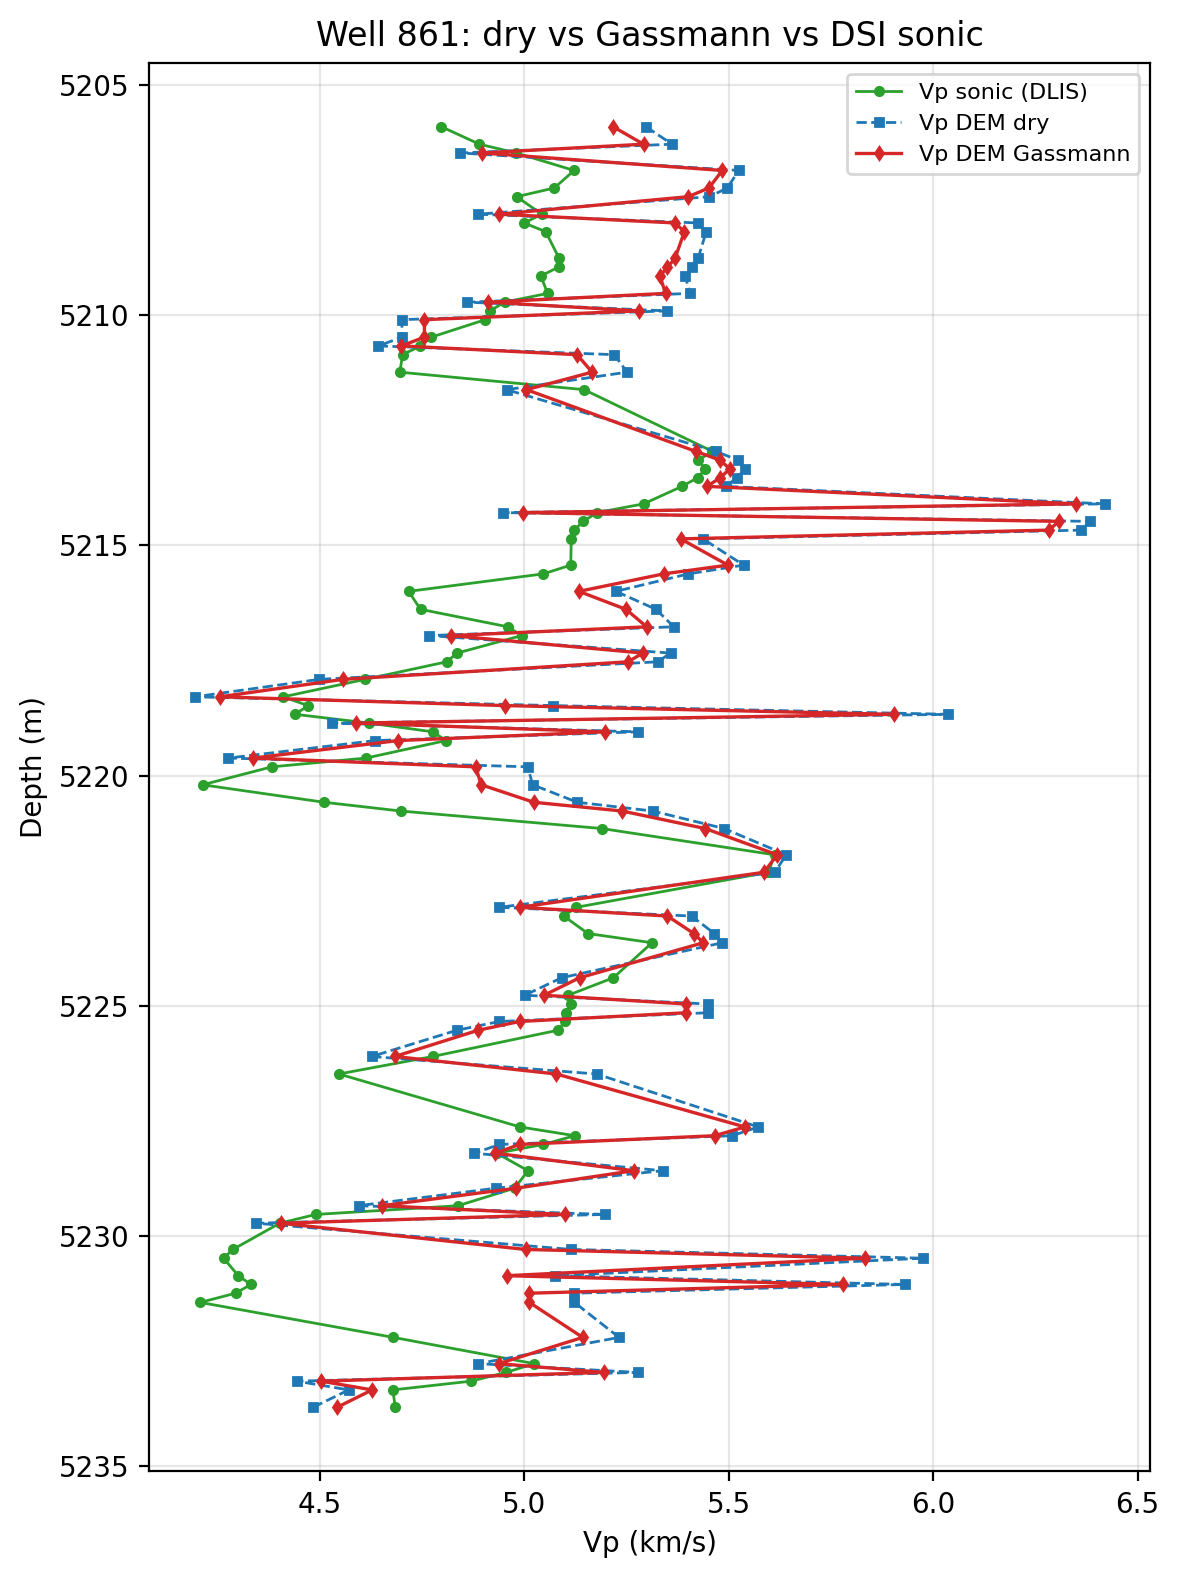
\includegraphics[width=0.78\linewidth]{figures/fig2_vp_dry_gassmann_sonic_depth}
  \caption{Referência da Etapa~2b: trilha de profundidade com \Vp{} sônico
           (verde), DEM a seco (azul tracejado) e DEM com Gassmann (vermelho).
           A saturação aproxima parcialmente o sônico, mas o viés
           $+0{,}27$~km/s persiste---motivação direta da Etapa~3.}
  \label{fig:gassmann_depth_ref}
\end{figure}

Na Figura~\ref{fig:gassmann_depth_ref}, trechos onde as três curvas se separam
mais (em especial faixas associadas às HFU~3 e~4 na discussão da Etapa~2)
coincidem com os maiores resíduos observados na Tabela~\ref{tab:hfu_compare}.
A Etapa~3 não altera a física Gassmann; aprende um corretor
$\widehat{\Delta V_{\mathrm{p}}}$ que desloca a trilha vermelha em direção
à verde, preservando a interpretação petrofísica do arcabouço DEM/SC.

\subsection{Sensibilidade ao regressor (herança da Etapa~1)}

Para verificar se a escolha do Random Forest é robusta, repetimos o protocolo
depth-block OOF com os \textbf{cinco regressores} da Etapa~1 (RF, Gradient
Boosting, XGBoost, MLP, regressão linear) mais \textbf{Ridge} (alternativa da
Etapa~1d), no mesmo alvo residual e nas mesmas oito \emph{features}.
A métrica decisiva é \Vp{} híbrida OOF versus DSI (MAPE e viés), não
apenas $R^2$ do resíduo.

A Tabela~\ref{tab:regressor_sensitivity} resume o desempenho global;
a Figura~\ref{fig:regressor_sensitivity} ordena os modelos por MAPE de \Vp{}
híbrida.

\begin{table}[H]
  \centering
  \caption{Sensibilidade ao regressor: resíduo OOF e \Vp{} híbrida versus DSI
           (87 linhas, depth-block CV, junho de 2026).}
  \label{tab:regressor_sensitivity}
  \small
  \begin{tabular}{lcccccc}
    \toprule
    Regressor & $R^2$ resíduo & RMSE res. (km/s) & MAPE híbr. (\%) &
    RMSE híbr. (km/s) & Viés híbr. (km/s) \\
    \midrule
    Regressão linear & 0,88 & 0,14 & 2,1 & 0,14 & $+0{,}00$ \\
    Random Forest & 0,79 & 0,18 & 2,8 & 0,18 & $+0{,}01$ \\
    Gradient Boosting & 0,69 & 0,22 & 3,0 & 0,22 & $+0{,}01$ \\
    XGBoost & 0,52 & 0,27 & 3,6 & 0,27 & $+0{,}02$ \\
    Ridge ($\alpha=1$) & 0,14 & 0,36 & 6,1 & 0,36 & $+0{,}04$ \\
    MLP & $-0{,}04$ & 0,40 & 6,5 & 0,40 & $+0{,}01$ \\
    \midrule
    Gassmann (baseline) & -- & -- & 7,3 & 0,48 & $+0{,}27$ \\
    \bottomrule
  \end{tabular}
\end{table}

\begin{figure}[H]
  \centering
  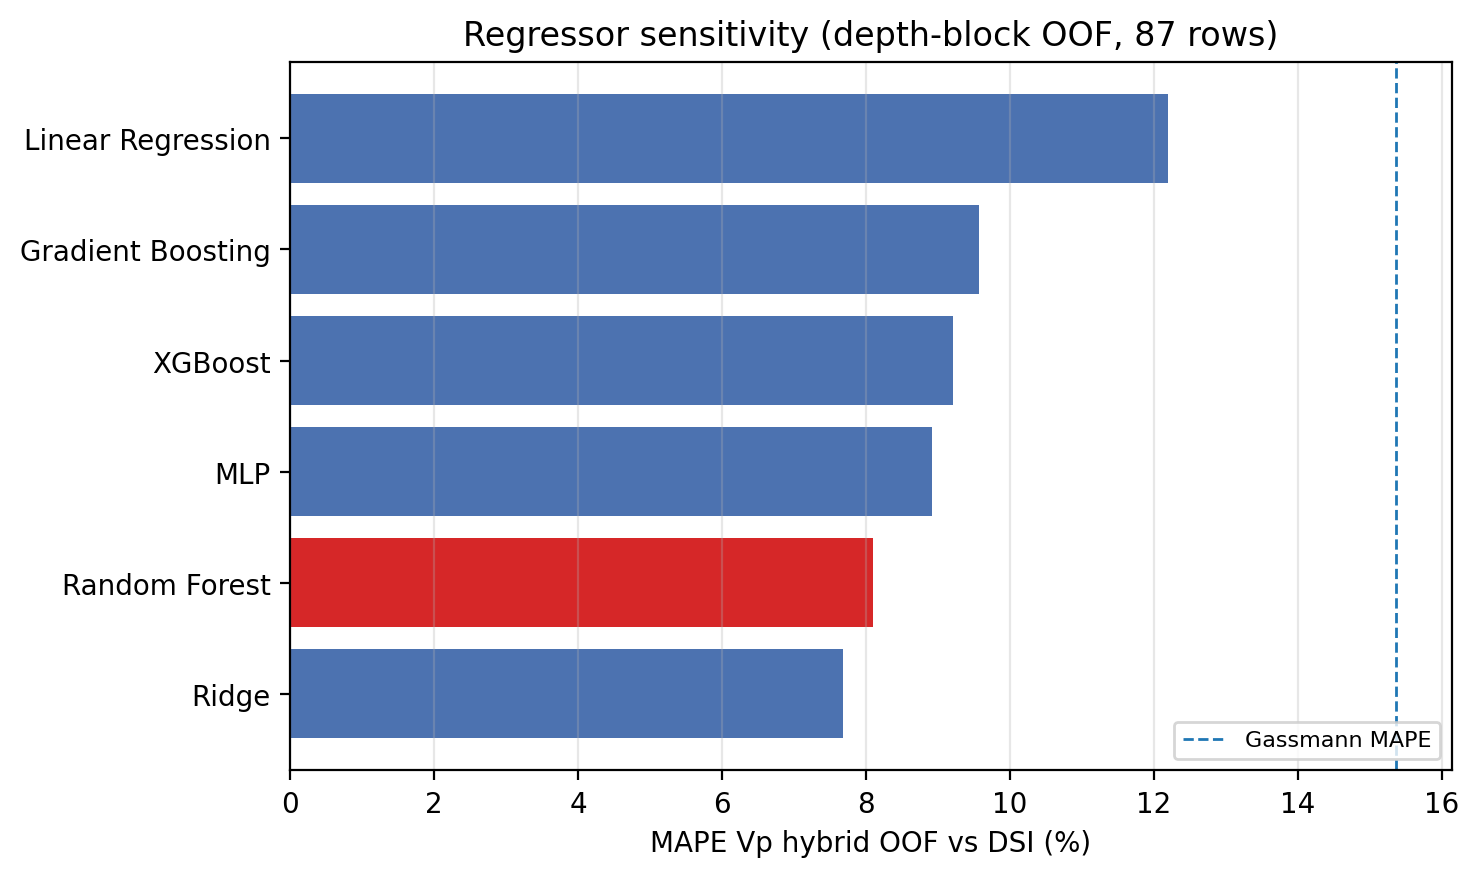
\includegraphics[width=0.82\linewidth]{figures/fig3_regressor_sensitivity_mape}
  \caption{MAPE de \Vp{} híbrida OOF versus DSI por regressor. Linha tracejada:
           baseline Gassmann (7,3\%). Todos os seis regressores ficam abaixo do
           baseline; RF (barra vermelha) permanece produto oficial e a regressão
           linear apresenta o menor MAPE nesta rodada.}
  \label{fig:regressor_sensitivity}
\end{figure}

A Figura~\ref{fig:regressor_depth_compare} exibe as trilhas de profundidade
comparativas: \Vp{} sônica (referência), Gassmann (baseline) e \Vp{}
híbrida OOF de cada regressor no mesmo intervalo 5205,91--5233,72~m.
A linha RF (vermelho) recebe traço mais grosso; demais regressores aparecem
com traço fino para não poluir a leitura.

\begin{figure}[H]
  \centering
  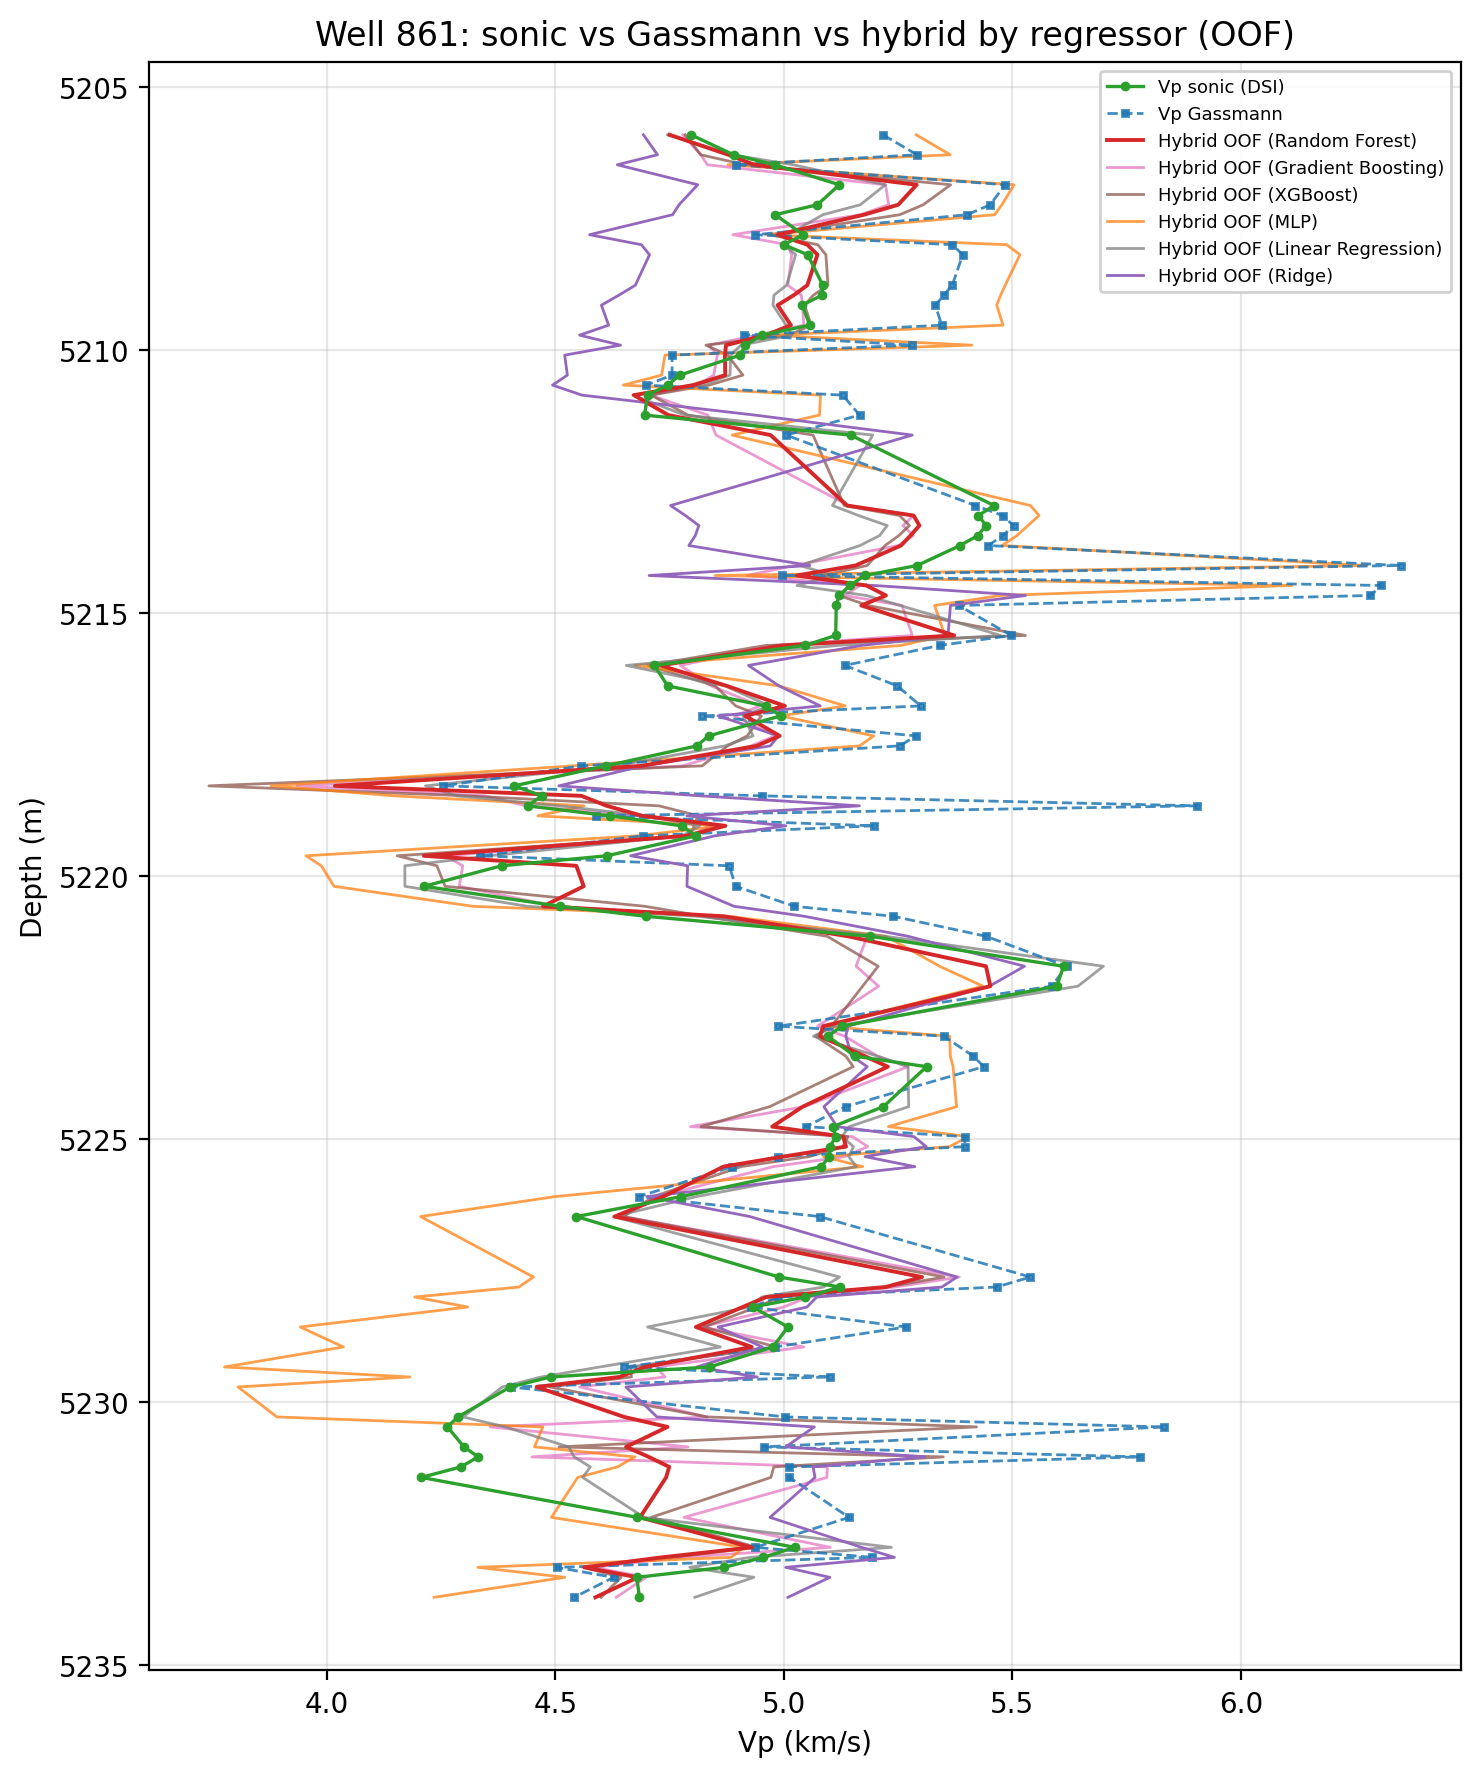
\includegraphics[width=0.85\linewidth]{figures/fig3_regressor_depth_comparison}
  \caption{Trilha de profundidade comparativa: \Vp{} sônico, Gassmann e híbrido
           OOF por regressor (depth-block CV, 87 linhas). RF, regressão linear
           e os dois \emph{boostings} colam na referência sônica; MLP e Ridge
           oscilam; Gassmann permanece sistematicamente acima.}
  \label{fig:regressor_depth_compare}
\end{figure}

Na Figura~\ref{fig:regressor_depth_compare}, todas as curvas híbridas deslocam
a trilha Gassmann em direção ao sônico, confirmando visualmente o ganho
da Tabela~\ref{tab:regressor_sensitivity}.
RF, regressão linear, Gradient Boosting e XGBoost praticamente se sobrepõem à
curva verde, inclusive nas excursões de baixa velocidade em torno de
5218 e 5230~m onde o Gassmann erra por mais de 1~km/s.
MLP (laranja) e Ridge (roxo) são os únicos que introduzem oscilações próprias,
com excursões abaixo de 4,0~km/s ausentes do sônico---razão pela qual seus
MAPE ficam no patamar de 6\%.

Na Tabela~\ref{tab:regressor_sensitivity}, a \textbf{regressão linear} alcança
o menor MAPE híbrido (2,1\%) e o maior $R^2$ no resíduo (0,88): o desvio
pós-Gassmann é, em boa medida, uma função quase linear da própria baseline
física e das curvas de perfil.
O \textbf{RF} vem logo atrás (MAPE 2,8\%, $R^2$ 0,79) com viés igualmente
desprezível ($+0{,}01$~km/s); adotamos o RF como corretor
oficial por consistência com a Etapa~1 e capacidade de interações não
lineares, mas a regressão linear é alternativa documentada e mais simples.
\textbf{Gradient Boosting} e \textbf{XGBoost} acompanham de perto
(MAPE 3,0\% e 3,6\%), o que mostra que o resultado não depende de um
algoritmo específico.
O \textbf{Ridge} ($\alpha = 1$) fica bem atrás da regressão linear que ele
penaliza (MAPE 6,1\% versus 2,1\%): como as \emph{features} não são
padronizadas antes do ajuste, a penalidade $L_2$ encolhe desproporcionalmente
os coeficientes das variáveis de menor escala e produz subajuste---efeito de
configuração, não evidência contra métodos regularizados.
O \textbf{MLP} é o pior do conjunto ($R^2$ residual levemente negativo, MAPE
6,5\%), coerente com o risco de instabilidade de redes com apenas 87 amostras.
Nenhum resultado altera a conclusão de que o corretor empírico reduz o gap
frente ao Gassmann; apenas refinam a escolha do algoritmo dentro do espectro
linear--não linear testado.

A Figura~\ref{fig:residual_scatter} exibe o ajuste OOF do RF (produto oficial)
no plano observado versus predito do resíduo.

\begin{figure}[H]
  \centering
  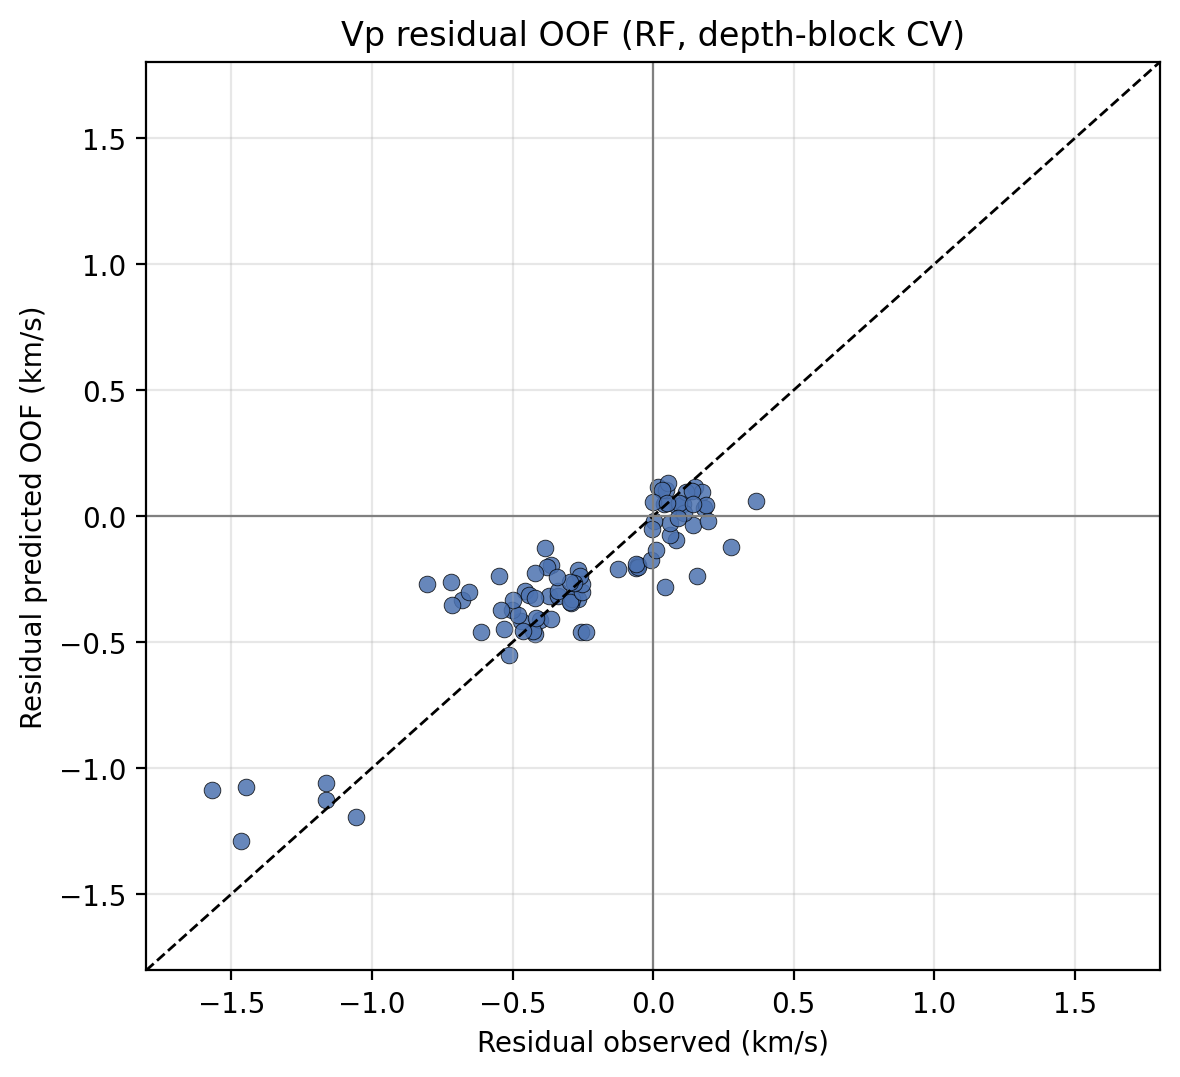
\includegraphics[width=0.72\linewidth]{figures/fig3_residual_oof_scatter}
  \caption{Resíduo observado versus predito (Random Forest, OOF por blocos de
           profundidade). A diagonal tracejada representa ajuste perfeito;
           desvios sistemáticos fora da diagonal indicariam viés no corretor ML.}
  \label{fig:residual_scatter}
\end{figure}

Na Figura~\ref{fig:residual_scatter}, a nuvem de pontos acompanha a diagonal
1:1 ao longo de toda a faixa, compatível com
$R^2_{\mathrm{OOF}} \approx 0{,}79$.
Resíduos observados \emph{negativos} (Gassmann acima do sônico) predominam,
coerente com o viés físico $+0{,}27$~km/s; o RF aprende a
atribuir correções negativas onde a física superestima \Vp{}.
A nuvem separa-se em dois regimes: um agrupamento denso entre $-0{,}6$ e
$+0{,}3$~km/s, que corresponde à maior parte do intervalo, e um punhado de
cinco pontos entre $-1{,}6$ e $-1{,}0$~km/s---as profundidades de HFU~4, onde
a calibração \emph{fallback} da Etapa~2 mais superestima \Vp{}.
O corretor recupera esses extremos com erro de 0,1--0,3~km/s, o que explica a
queda de MAPE concentrada naquela unidade
(Tabela~\ref{tab:hfu_compare}), mas cinco pontos não sustentam extrapolação:
qualquer profundidade nova com resíduo dessa magnitude estaria fora do suporte
efetivo de treino.

\subsection{Trilhas em profundidade: antes e depois do corretor ML}

A Figura~\ref{fig:hybrid_depth} confronta as três trilhas ao longo de
5205,91--5233,72~m \emph{após} a Etapa~3: \Vp{} sônica (referência),
\Vp{} Gassmann (baseline física, idêntica à linha vermelha da
Figura~\ref{fig:gassmann_depth_ref}) e \Vp{} híbrida OOF (produto desta etapa).

\begin{figure}[H]
  \centering
  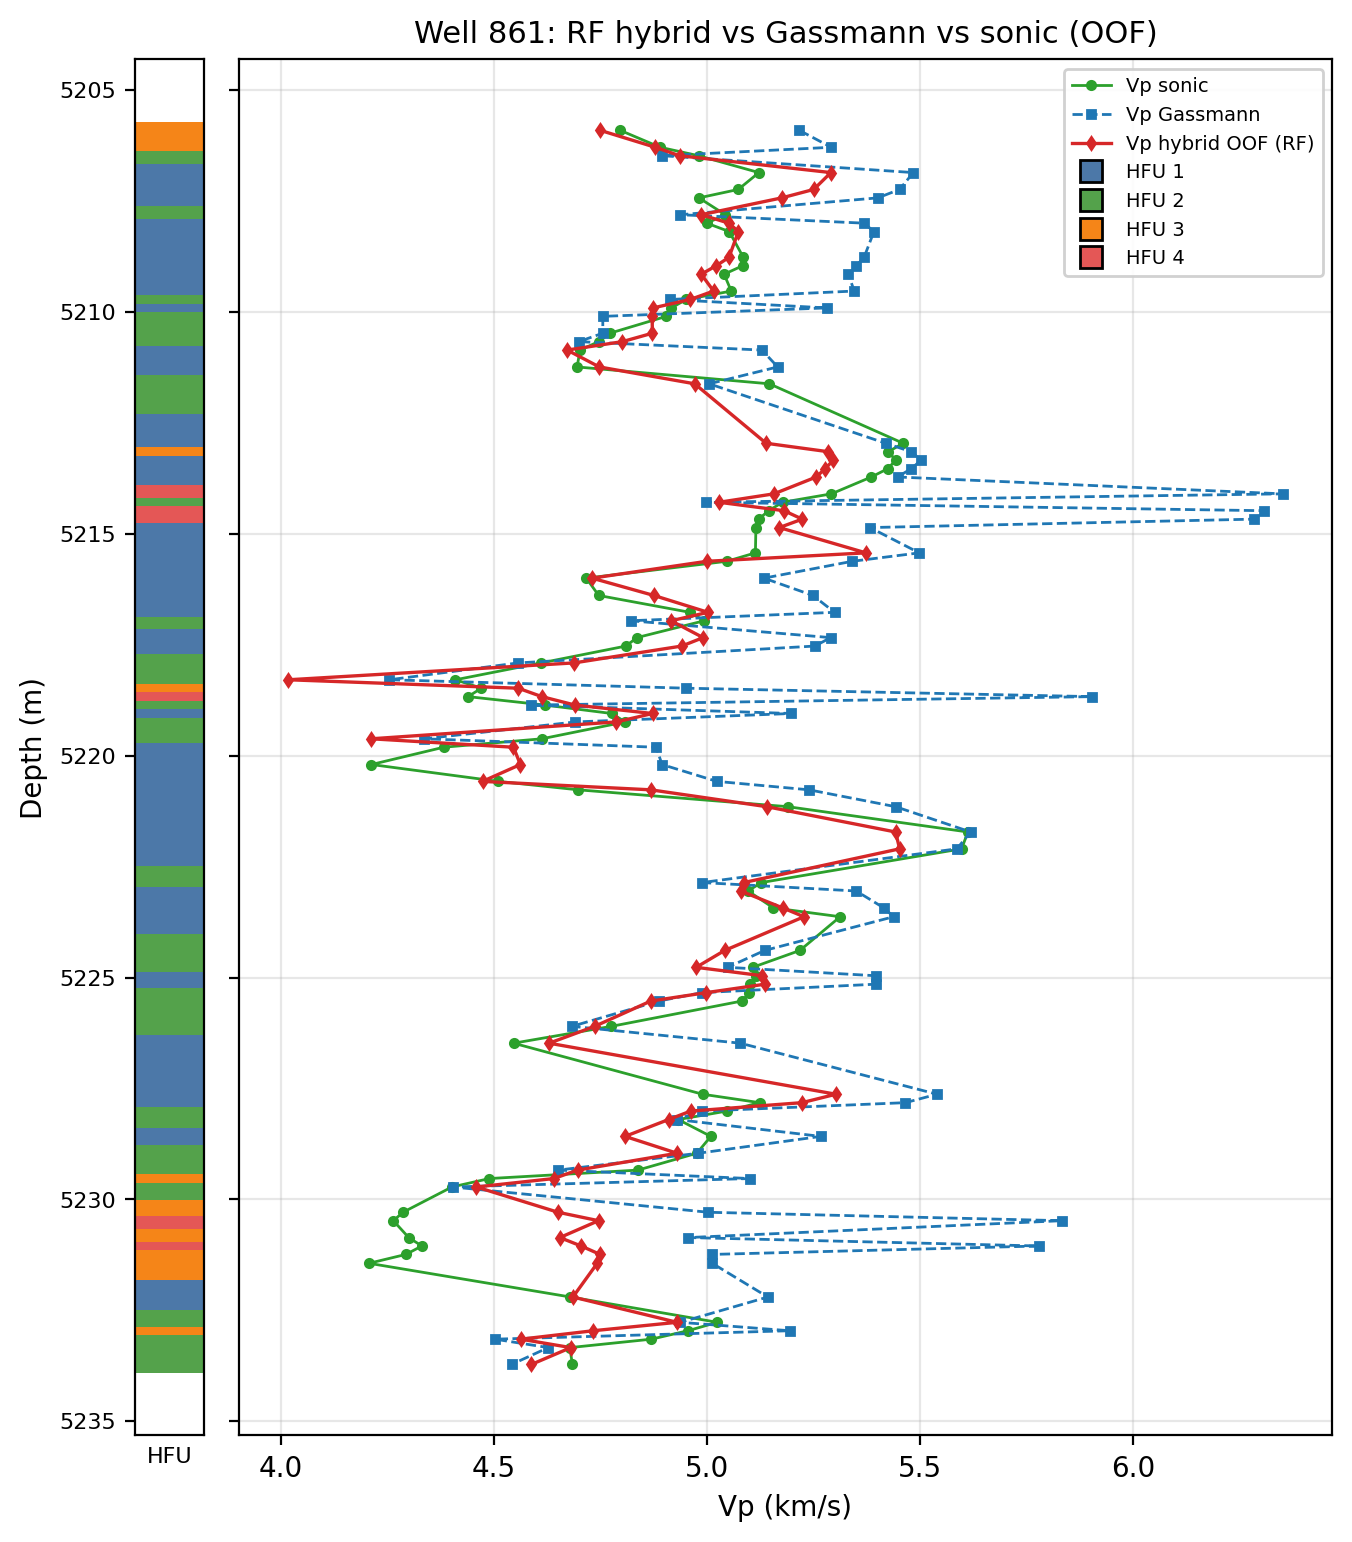
\includegraphics[width=0.78\linewidth]{figures/fig3_vp_hybrid_depth_hfu}
  \caption{Trilha de profundidade pós-Etapa~3: \Vp{} sônico (DSI), Gassmann
           (Etapa~2b) e híbrido OOF (Etapa~3), com faixa lateral colorida pela
           HFU de laboratório em cada amostra. As HFUs são intercaladas ao
           longo da coluna (não formam blocos contínuos). Comparar com a
           Figura~\ref{fig:gassmann_depth_ref}: o corretor ML aproxima a trilha
           física do sônico sem substituir a baseline Gassmann.}
  \label{fig:hybrid_depth}
\end{figure}

A Figura~\ref{fig:hybrid_ridge_depth} repete o mesmo painel para o
\textbf{Ridge} ($\alpha = 1$), variante penalizada com MAPE híbrido de 6,1\%
e viés $+0{,}04$~km/s.

\begin{figure}[H]
  \centering
  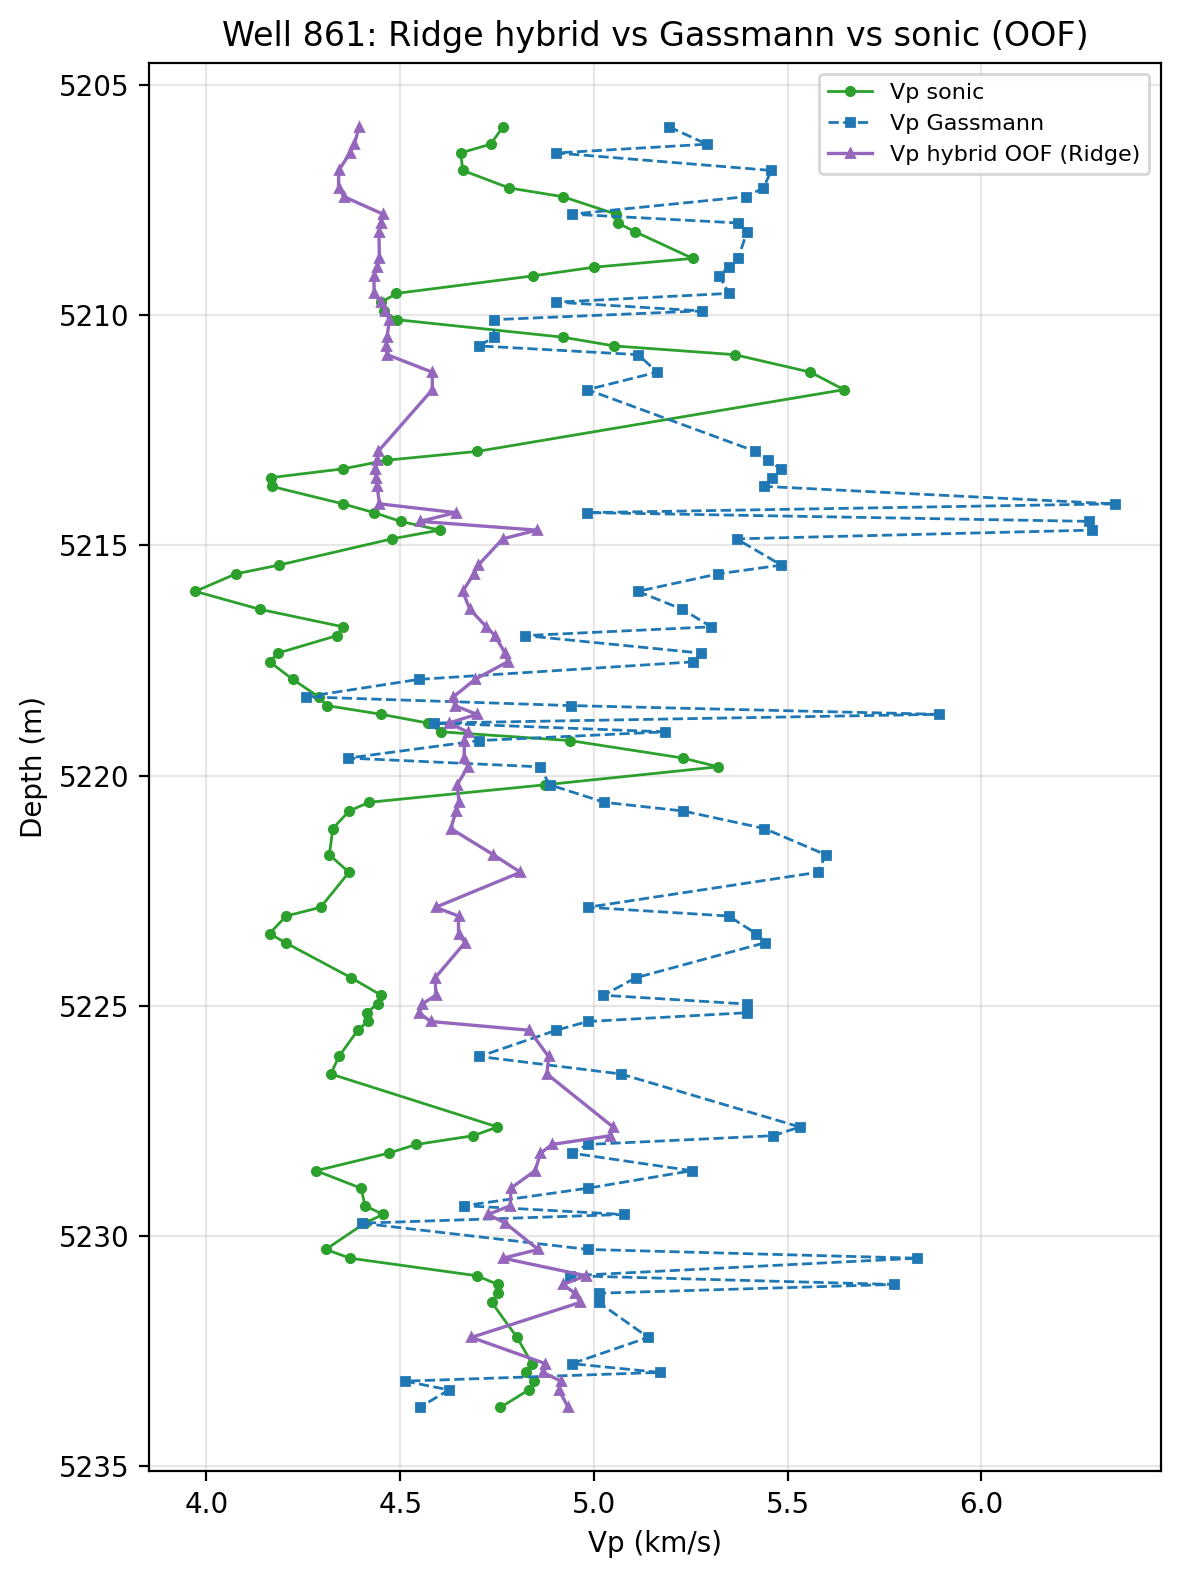
\includegraphics[width=0.78\linewidth]{figures/fig3_vp_hybrid_ridge_depth}
  \caption{Trilha de profundidade pós-Etapa~3 (Ridge OOF): \Vp{} sônico (DSI),
           Gassmann (Etapa~2b) e híbrido Ridge. MAPE 6,1\% e viés $+0{,}04$~km/s
           versus DSI; comparar com a Figura~\ref{fig:hybrid_depth} (RF, MAPE 2,8\%,
           viés $+0{,}01$~km/s).}
  \label{fig:hybrid_ridge_depth}
\end{figure}

Na Figura~\ref{fig:hybrid_depth}, a linha Gassmann (azul tracejada) reproduz o
viés positivo já visível na Figura~\ref{fig:gassmann_depth_ref}, com picos
acima de 6~km/s em torno de 5214 e 5219~m que não têm contrapartida no sônico.
A trilha híbrida (vermelha) acompanha a sônica (verde) ao longo de quase todo o
intervalo, inclusive nesses picos.
As discrepâncias remanescentes concentram-se em 5228--5232~m, onde o sônico
desce a 4,2~km/s e o híbrido para em torno de 4,7~km/s: nesses segmentos
recomenda-se revisão geológica (facies, fraturas, qualidade do
casamento DSI) antes de exportar \Vp{} híbrida para produto de perfil.
Na Figura~\ref{fig:hybrid_ridge_depth}, a curva híbrida Ridge (roxa) mostra o
padrão oposto ao desejado nos extremos: subcorrige na base do intervalo e
sobrecorrige no topo (5205--5210~m), afastando-se do sônico para valores
abaixo de 4,5~km/s---assinatura visual do subajuste discutido na
Tabela~\ref{tab:regressor_sensitivity}.
A leitura conjunta das duas figuras de profundidade---Etapa~2b como diagnóstico,
Etapa~3 como correção---evita interpretar o ganho do ML como substituição
da cadeia física.

\subsection{Desempenho por HFU}
\label{sec:resultados_hfu}

A Tabela~\ref{tab:hfu_compare} detalha MAPE e viés por unidade hidrodinâmica
de fluxo, comparando Gassmann e híbrido OOF.
A HFU vem de laboratório (mesma segmentação da calibração DEM/SC);
a análise é \emph{pós-hoc}, não influencia o treino.

\textbf{Leitura correta da estratificação.}
As HFUs \textbf{não} formam intervalos contíguos de profundidade: ao longo
da coluna elas são \textbf{intercaladas} (faixa lateral da
Figura~\ref{fig:hybrid_depth}).
Os números da Tabela~\ref{tab:hfu_compare} agrupam as 87 amostras pelo
\emph{rótulo} de HFU de cada linha---não são MAPE de ``zonas''
$z\in[z_a,z_b]$ associadas a uma única HFU.
Por isso a tabela e o gráfico de profundidade respondem a perguntas
diferentes: a tabela resume erro por classe petrofísica; o gráfico mostra
\emph{onde} essas classes aparecem (misturadas) e como as trilhas se
comportam linha a linha.
Não se deve confundir essa estratificação com os blocos de profundidade
do OOF ($B_0,B_1,B_2$), que são contíguos por construção.

\begin{table}[H]
  \centering
  \caption{MAPE e viés de \Vp{} versus DSI por HFU: Gassmann versus híbrido OOF
           (agregação por rótulo de amostra; HFUs intercaladas em profundidade).}
  \label{tab:hfu_compare}
  \begin{tabular}{ccccc}
    \toprule
    HFU & $n$ & MAPE Gass. (\%) & MAPE híbr. (\%) & Viés Gass. / híbr. (km/s) \\
    \midrule
    1 & 42 & 6,8 & 2,2 & $+0{,}33$ / $+0{,}02$ \\
    2 & 29 & 2,2 & 2,3 & $-0{,}11$ / $-0{,}09$ \\
    3 & 10 & 11,5 & 5,4 & $+0{,}51$ / $+0{,}15$ \\
    4 & 6  & 28,1 & 4,8 & $+1{,}31$ / $+0{,}17$ \\
    \bottomrule
  \end{tabular}
\end{table}

Na Tabela~\ref{tab:hfu_compare}, o ganho mais expressivo ocorre na
HFU~4 (MAPE 28,1\% $\rightarrow$ 4,8\%; viés
$+1{,}31 \rightarrow +0{,}17$~km/s) e na HFU~3
(11,5\% $\rightarrow$ 5,4\%; viés $+0{,}51 \rightarrow +0{,}15$~km/s).
A HFU~4, calibrada por \emph{fallback} na Etapa~2 (sem plugs), superestimava
\Vp{} em mais de 1,3~km/s em média (predição $\approx 6{,}08$ versus
sônica $\approx 4{,}77$~km/s); o híbrido recalibra essas \emph{amostras}
para perto do DSI, mas o suporte de apenas seis pontos e a validação OOF
no mesmo poço impõem cautela---o resultado é \emph{promissor}, não definitivo.
A HFU~1 concentra 42 das 87 amostras e, com MAPE físico já moderado (6,8\%),
cai para 2,2\% com viés praticamente nulo; por ser a classe majoritária, é ela
que puxa o MAPE global para 2,8\%.
A HFU~2 é o contraexemplo instrutivo: a física pura já entregava 2,2\% de MAPE
com viés levemente \emph{negativo} ($-0{,}11$~km/s), e o corretor não melhora
nada---passa a 2,3\%.
Ou seja, o ML não degrada onde a física já fecha, mas também não tem o que
extrair ali; o ganho vem inteiramente das unidades mal calibradas.
Essa leitura reforça que o corretor está compensando deficiência de
calibração DEM/SC por HFU, não descobrindo física nova.
Em outras palavras: a falta de plugs na HFU~4 explica o gap grande do
\textbf{Gassmann} frente ao sônico; \textbf{não} explica os
$\approx 5\%$ de MAPE que restam no híbrido após a correção---esses
remanescentes são erro residual do corretor, não o mesmo mecanismo do
viés físico original.

\subsection{CLP-CSGM sobre resíduo \Vp{} (Etapa~3b)}
\label{sec:clp_vp_residual}

Para alinhar a Etapa~3 ao arcabouço CLP-CSGM da Etapa~1f, implementamos
três variantes que modelam o resíduo em \textbf{janelas deslizantes}
($L=16$, passo~1) em vez de regressão pontual:

\begin{equation}
  V_{\mathrm{p,hybrid}} = V_{\mathrm{p,Gassmann}} + G(\hat{\mathbf{z}}),
  \label{eq:clp_vp_hybrid}
\end{equation}

onde $G$ é o decoder do autoencoder treinado em janelas de
$\Delta V_{\mathrm{p}} = V_{\mathrm{p,sonic}} - V_{\mathrm{p,Gassmann}}$,
e $\hat{\mathbf{z}}$ provém do prior Ridge $h(\mathbf{u})$ sobre os oito
canais densos da janela (sete wireline mais \Vp{} Gassmann) ou de
refinamento com medidas esparsas nos dez plugs CT (análogo à variante~B
residual de \philab{} na Etapa~1f, mas com baseline Gassmann em vez de RF).

As três variantes testadas (validação depth-block OOF, stitch
\emph{uniform\_mean}):

\begin{itemize}
  \item \textbf{CLP Ridge prior ($m{=}0$):}
        $\mathbf{z}_0 = h(\mathbf{u})$, sem termo de consistência em teste;
  \item \textbf{CLP zero residual ($m{=}0$):}
        $\mathbf{z}_0 = \mathrm{encode}(\mathbf{0})$, confia na física Gassmann;
  \item \textbf{CLP plug sparse $b$:}
        $\mathbf{z}_0 = \mathrm{encode}(\mathbf{0})$ com
        $b = M\,\Delta V_{\mathrm{p}}$ apenas nos índices-plug da janela
        ($\lambda^\star = 0{,}001$ na validação interna).
\end{itemize}

A Tabela~\ref{tab:clp_compare_global} compara Gassmann, RF híbrido e as
três variantes CLP contra o DSI (87/87).

\begin{table}[H]
  \centering
  \caption{Comparação global: Gassmann, RF híbrido OOF e CLP-CSGM residual
           (Etapa~3b, depth-block CV, junho de 2026).}
  \label{tab:clp_compare_global}
  \begin{tabular}{lccc}
    \toprule
    Modelo & MAPE (\%) & RMSE (km/s) & Viés (km/s) \\
    \midrule
    Gassmann (baseline) & 7,3 & 0,48 & $+0{,}27$ \\
    RF híbrido OOF & 2,8 & 0,18 & $+0{,}01$ \\
    CLP Ridge prior ($m{=}0$) & 6,5 & 0,44 & $+0{,}06$ \\
    CLP zero residual ($m{=}0$) & 6,7 & 0,44 & $+0{,}19$ \\
    CLP plug sparse $b$ & 6,3 & 0,43 & $+0{,}18$ \\
    \bottomrule
  \end{tabular}
\end{table}

Na Tabela~\ref{tab:clp_compare_global}, \textbf{nenhuma variante CLP supera o RF}
pontual (2,8\% MAPE).
As três ficam agrupadas em 6,3--6,7\%, ou seja, batem o Gassmann por menos de
um ponto percentual e perdem do RF por cerca de 3,6 pontos.
O agrupamento é informativo: a variante que usa medidas esparsas nos plugs
(6,3\%) e a que simplesmente assume resíduo nulo (6,7\%) praticamente empatam,
o que indica que o ganho das variantes CLP vem sobretudo do
\emph{prior} do autoencoder e do stitch por sobreposição, não da informação
esparsa injetada em $b$.
O prior Ridge em janelas ($m{=}0$) é o que mais reduz o viés
($+0{,}06$~km/s, o melhor entre as CLP), mas não converte isso em MAPE porque
troca viés por dispersão: apesar do viés quase três vezes menor que o da variante
plug sparse, seu RMSE é ligeiramente maior (0,442 contra 0,427~km/s).
No conjunto, o AE em $\Delta V_{\mathrm{p}}$ com reconstrução por janelas não
captura a mesma informação local que o RF nas oito \emph{features} pontuais.
A variante plug sparse aproxima-se do RF na HFU~2
(Tabela~\ref{tab:clp_hfu_compare}), mas falha na HFU~4
(MAPE $\approx 26\%$ versus 4,8\% no RF), onde o suporte de seis amostras
e a escassez de plugs na janela limitam o refinamento inverso---na prática,
a variante CLP herda quase intacto o erro físico daquela unidade.

\begin{table}[H]
  \centering
  \caption{MAPE e viés por HFU: melhor CLP (plug sparse $b$) versus RF híbrido OOF.}
  \label{tab:clp_hfu_compare}
  \begin{tabular}{ccccc}
    \toprule
    HFU & $n$ & MAPE RF (\%) & MAPE CLP plug (\%) &
    Viés RF / CLP (km/s) \\
    \midrule
    1 & 42 & 2,2 & 4,8 & $+0{,}02$ / $+0{,}21$ \\
    2 & 29 & 2,3 & 3,3 & $-0{,}09$ / $-0{,}16$ \\
    3 & 10 & 5,4 & 9,8 & $+0{,}15$ / $+0{,}43$ \\
    4 & 6  & 4,8 & 25,9 & $+0{,}17$ / $+1{,}20$ \\
    \bottomrule
  \end{tabular}
\end{table}

Na Tabela~\ref{tab:clp_hfu_compare}, o RF vence em todas as quatro unidades,
mas a distância varia muito.
Nas HFU~1 e~2, onde o baseline físico já era razoável, a diferença é de
2--3 pontos percentuais; na HFU~4 ela salta para 21 pontos.
Isto é, a desvantagem do CLP concentra-se exatamente onde o corretor precisa
aplicar uma correção grande e localizada: a reconstrução por janelas
suaviza o resíduo e não consegue reproduzir o degrau de mais de 1~km/s da
HFU~4, enquanto o RF pontual o reproduz ponto a ponto.

A Figura~\ref{fig:clp_mape} ordena os modelos por MAPE; a
Figura~\ref{fig:clp_depth} confronta trilhas de profundidade RF versus CLP
Ridge prior; a Figura~\ref{fig:clp_three_methods} inclui a variante plug
sparse junto ao RF.

\begin{figure}[H]
  \centering
  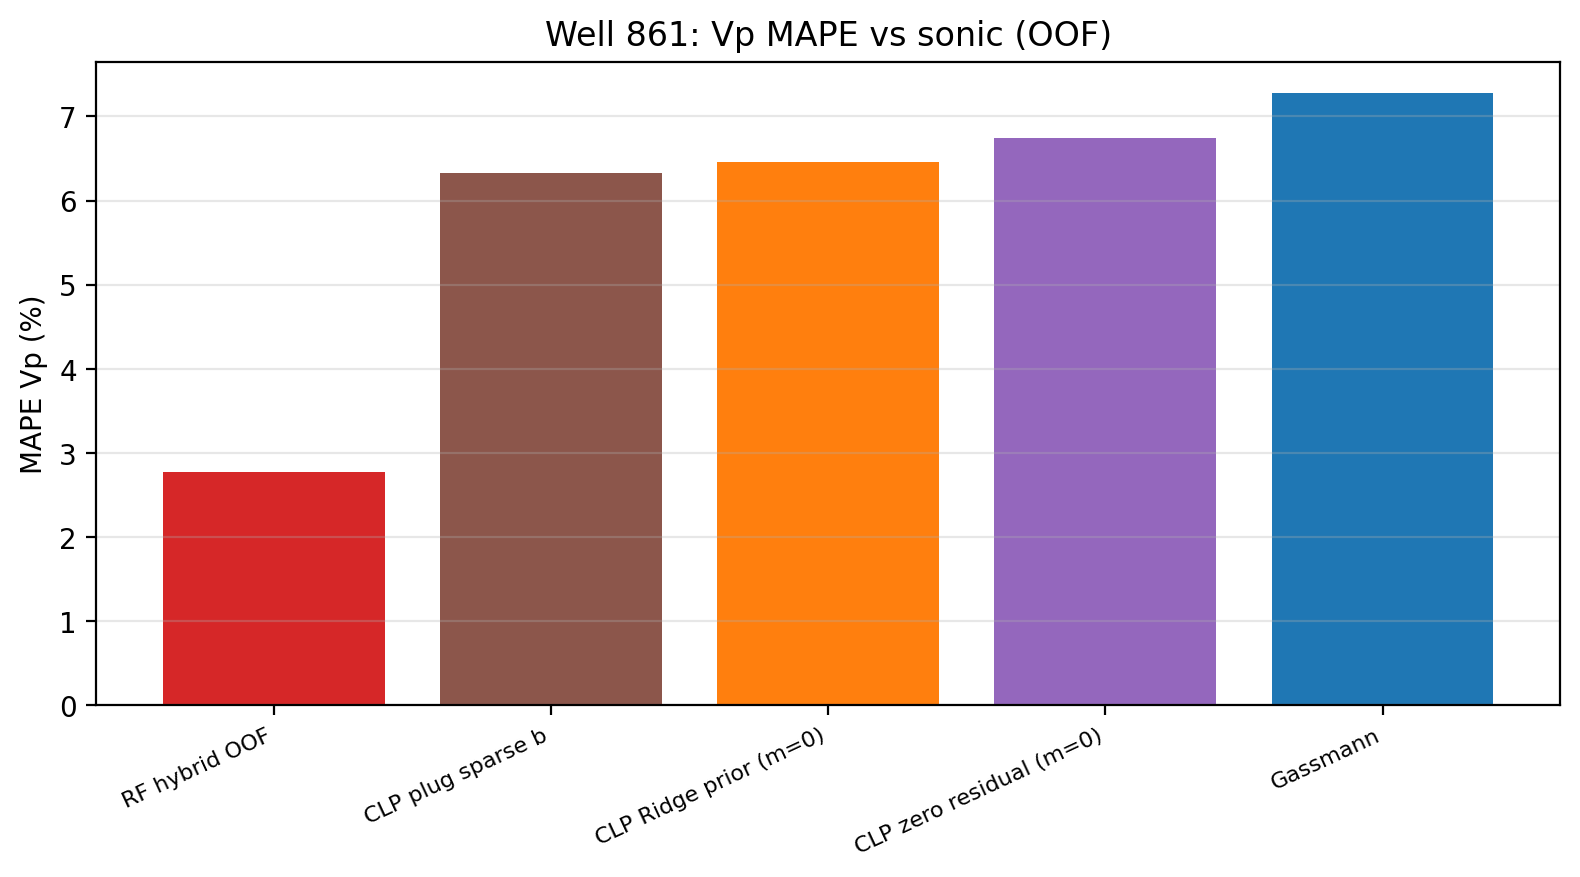
\includegraphics[width=0.82\linewidth]{figures/fig3_clp_comparison_mape}
  \caption{MAPE de \Vp{} versus DSI: Gassmann, RF híbrido OOF e três variantes
           CLP-CSGM residual (Etapa~3b). O RF pontual permanece o melhor
           corretor neste poço.}
  \label{fig:clp_mape}
\end{figure}

\begin{figure}[H]
  \centering
  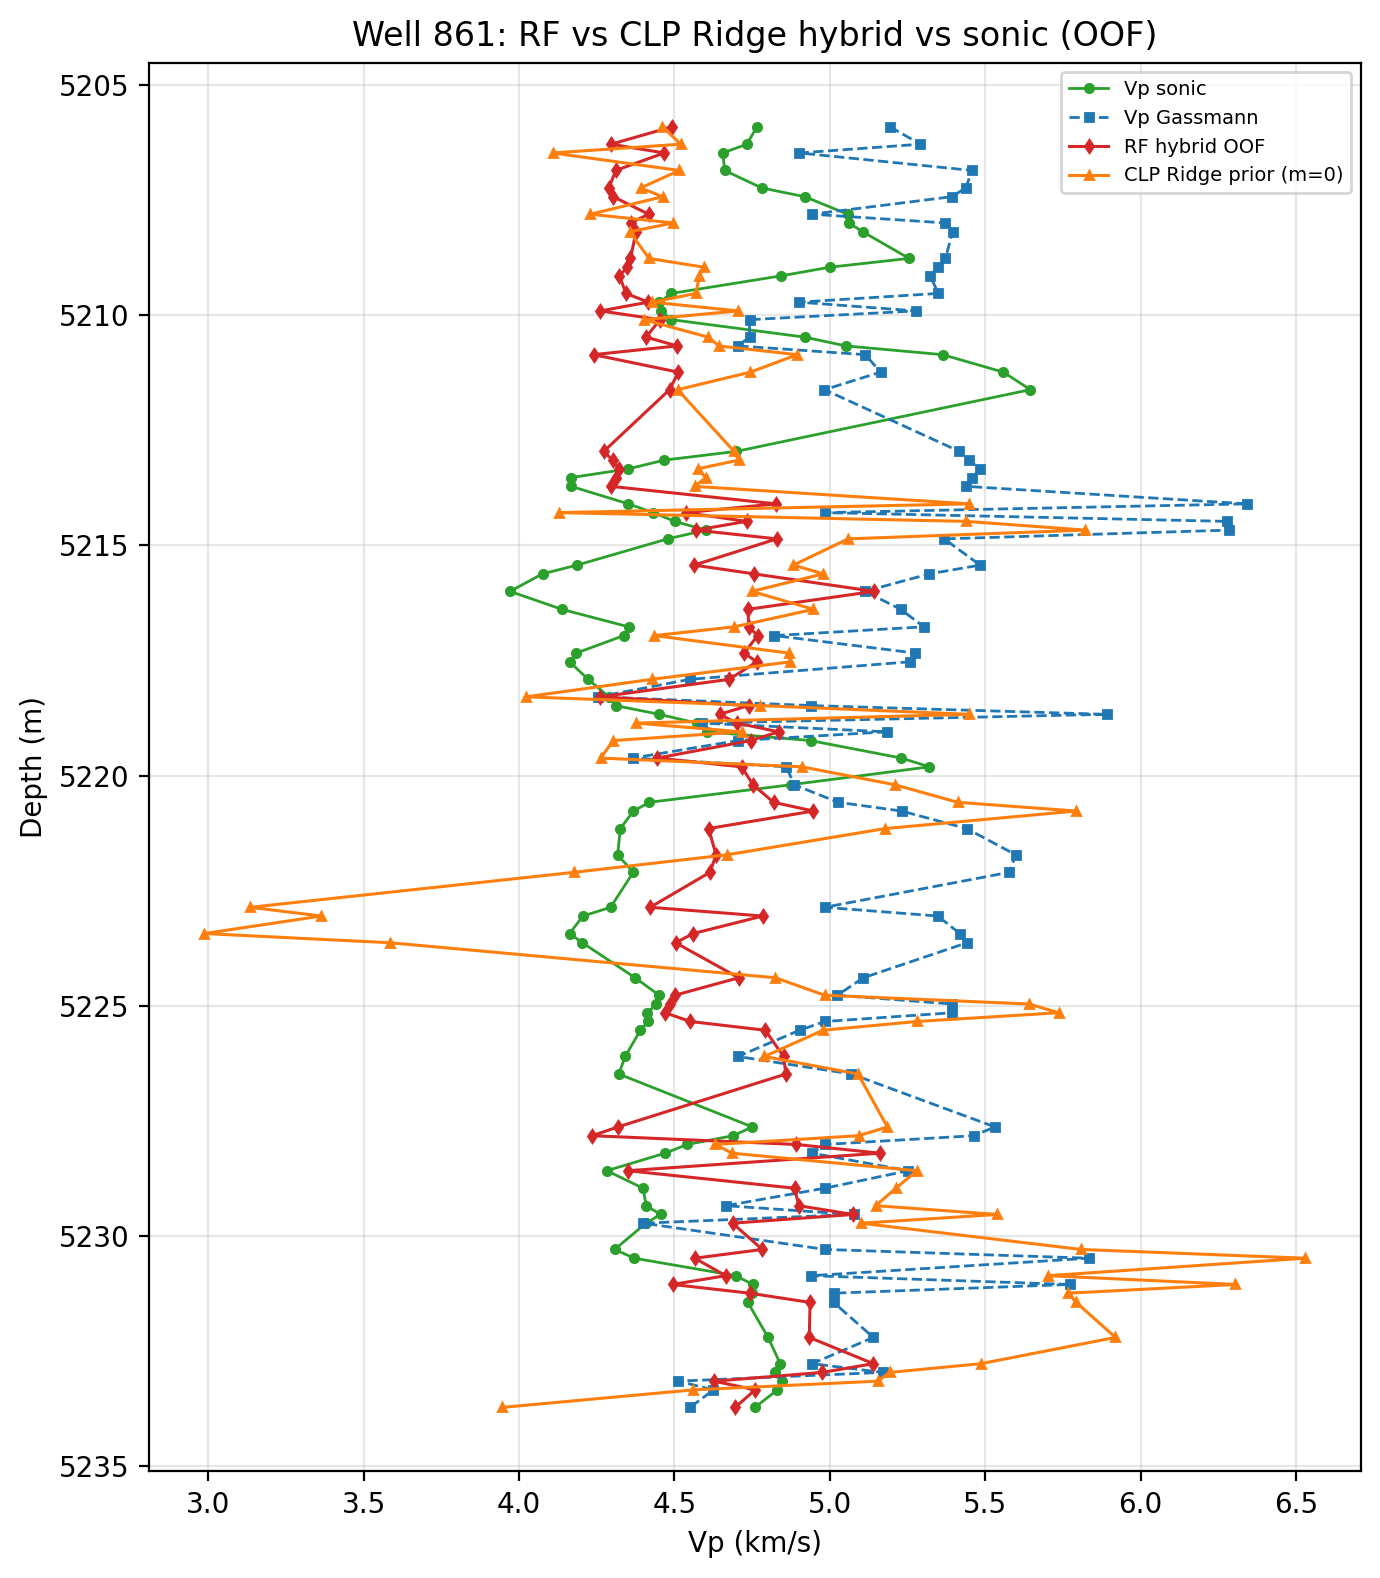
\includegraphics[width=0.85\linewidth]{figures/fig3_clp_vp_hybrid_depth}
  \caption{Trilha de profundidade: sônico, Gassmann, RF híbrido OOF e CLP
           Ridge prior ($m{=}0$). O CLP suaviza o resíduo em janelas, mas
           não aproxima o DSI com a mesma fidelidade do RF.}
  \label{fig:clp_depth}
\end{figure}

\begin{figure}[H]
  \centering
  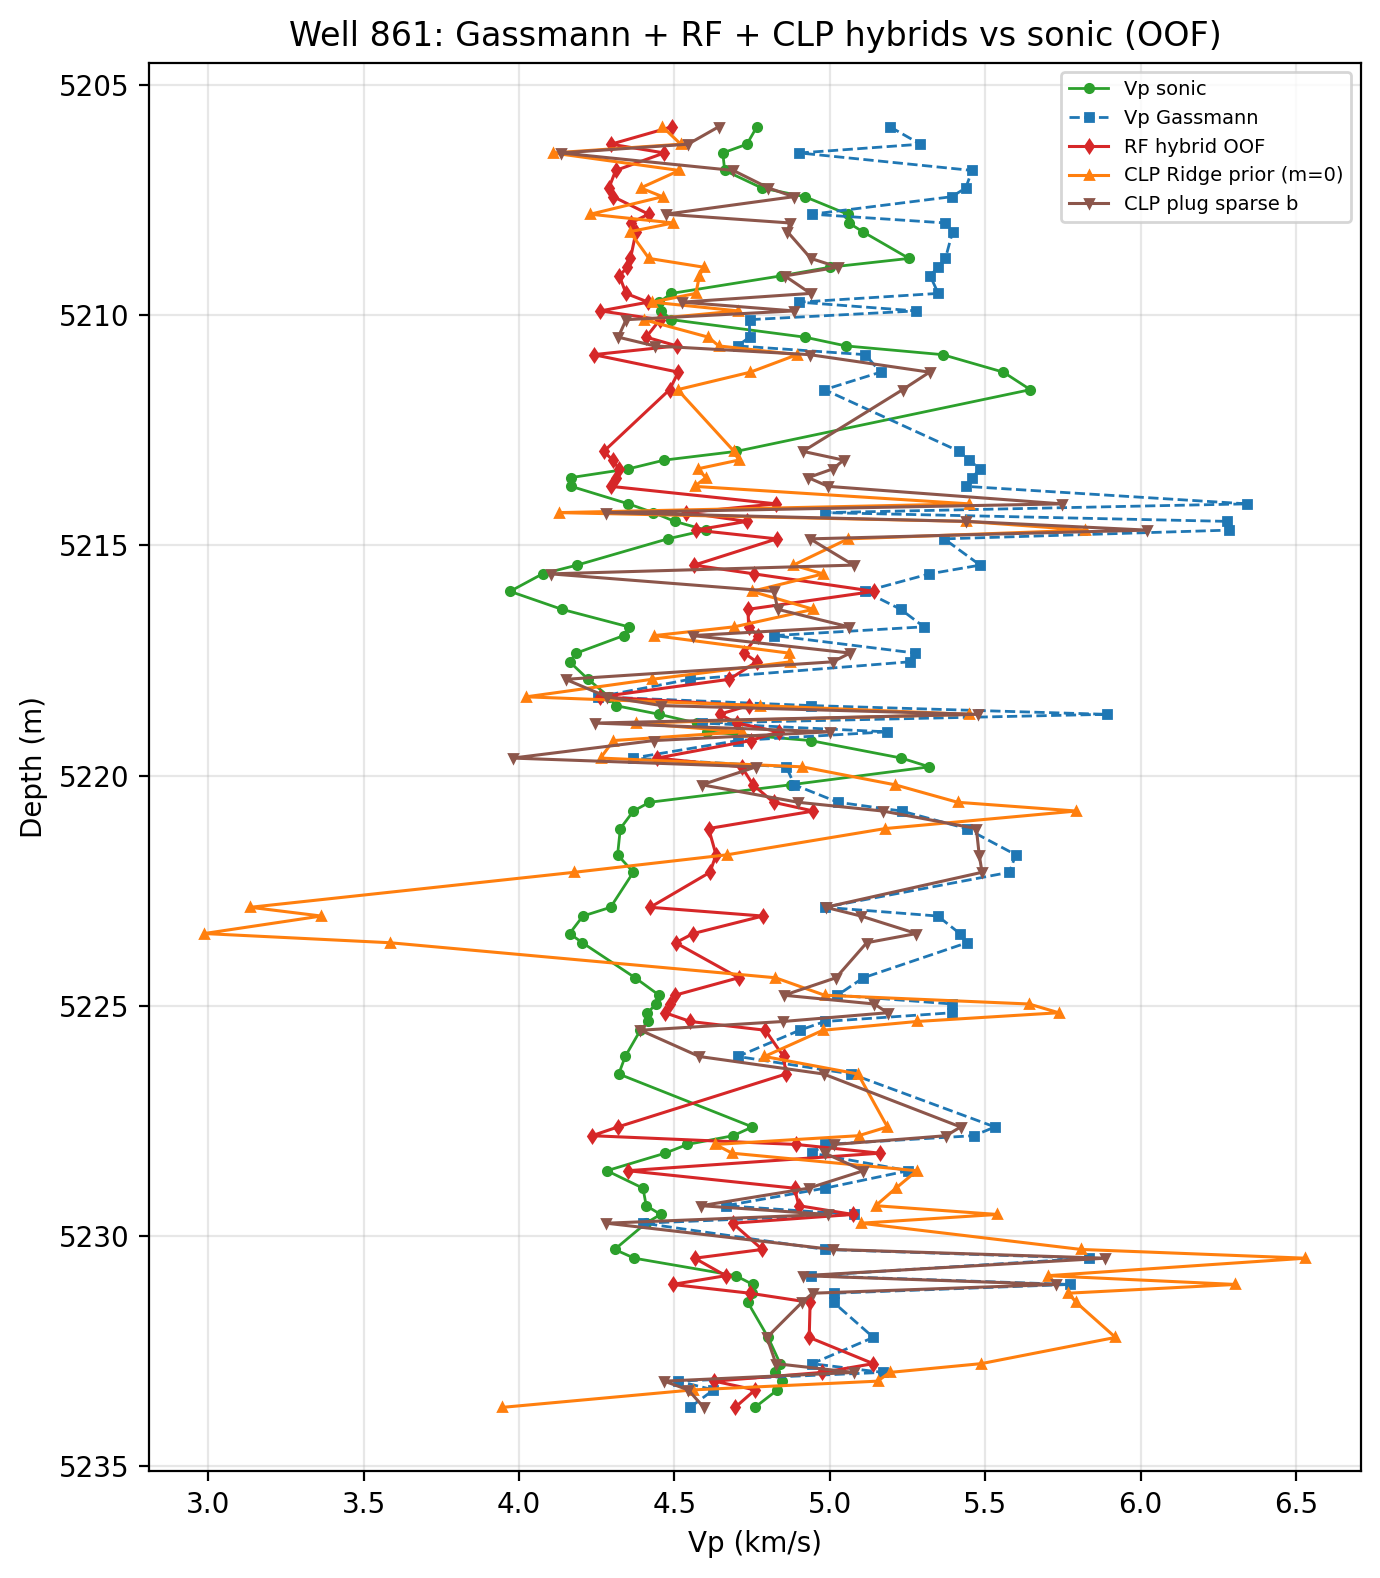
\includegraphics[width=0.85\linewidth]{figures/fig3_clp_three_methods_depth}
  \caption{Comparação de híbridos OOF: RF, CLP Ridge prior e CLP plug sparse
           $b$ versus sônico e Gassmann.}
  \label{fig:clp_three_methods}
\end{figure}

\begin{figure}[H]
  \centering
  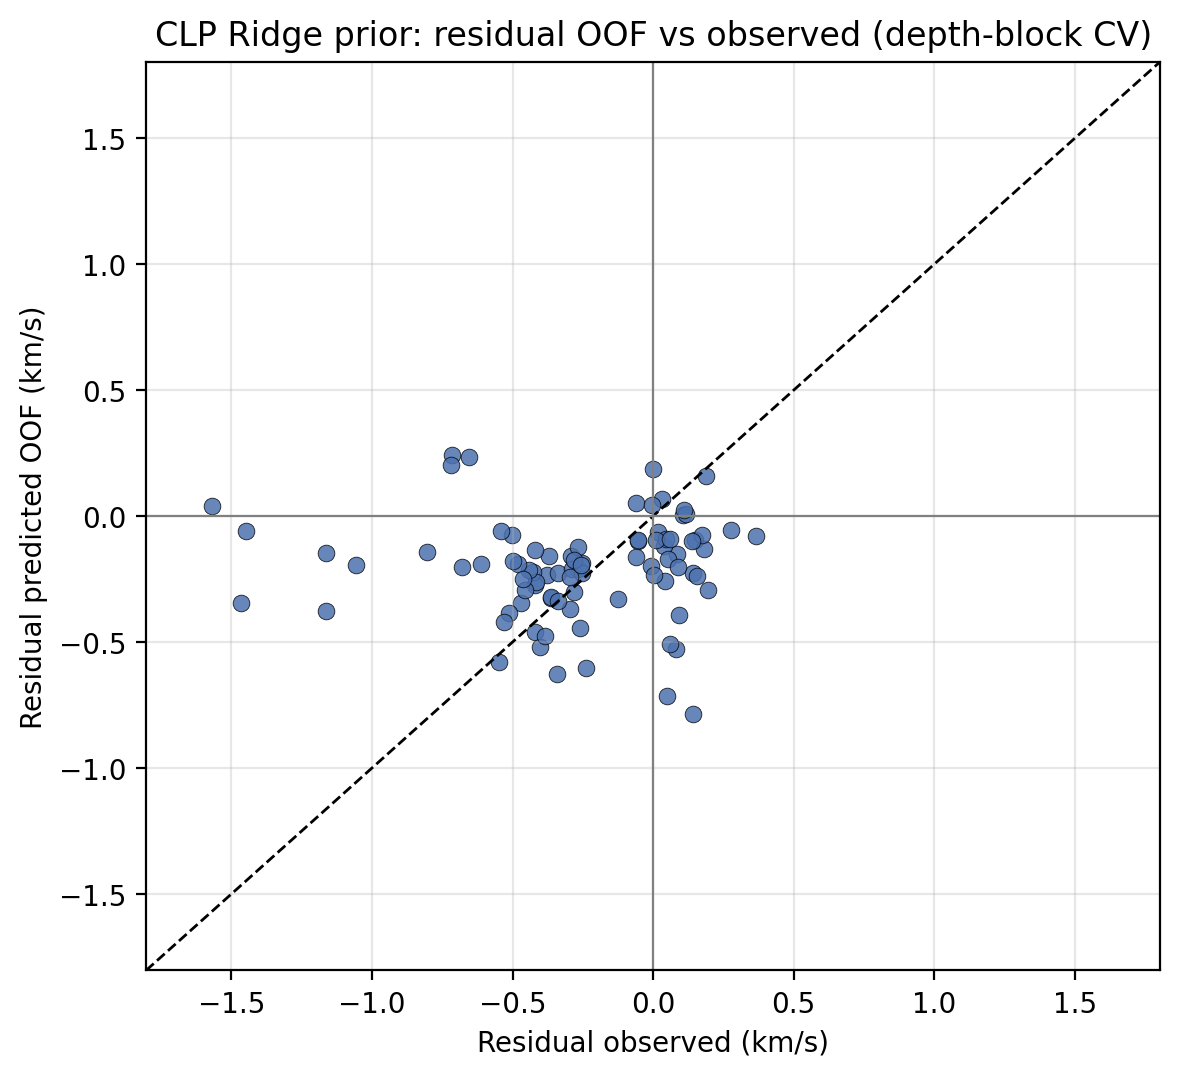
\includegraphics[width=0.72\linewidth]{figures/fig3_clp_residual_scatter}
  \caption{Resíduo observado versus predito OOF (CLP Ridge prior, depth-block CV).}
  \label{fig:clp_residual_scatter}
\end{figure}

\textbf{Recomendação Etapa~3b:} manter o RF (ou a regressão linear, 2,1\% MAPE)
como corretor residual principal quando o sônico supervisiona o treino em
todo o intervalo; reservar CLP-CSGM para cenários com
\textbf{medidas esparsas de calibração} em $b$ (Seção~\ref{sec:rho_sweep}).

\subsection{Sensibilidade $\rho$: calibração esparsa (Etapa~3c)}
\label{sec:rho_sweep}

Para quantificar \emph{quanta} informação esparsa o CLP exige para competir
com o RF oracle, varremos a fração $\rho$ de profundidades com
$\Delta V_{\mathrm{p}}$ conhecido em $b$ (protocolo depth-block OOF, igual
número de pontos de calibração para CLP e RF sparse).

\begin{itemize}
  \item \textbf{CLP sparse $b$:} $b = M\,\Delta V_{\mathrm{p}}$ nos índices
        calibrados; $\mathbf{z}_0 = \mathrm{encode}(\mathbf{0})$.
  \item \textbf{RF sparse:} treina \emph{somente} nas profundidades
        calibradas do bloco de treino; prediz todo o bloco de teste.
  \item \textbf{Referência:} RF oracle (treino denso, 2,9\% MAPE) e Gassmann.
\end{itemize}

Em $\rho=10/87$ (dez plugs fixos), o CLP leva vantagem modesta sobre o RF
sparse (6,5\% contra 7,5\% de MAPE), mas ambos ficam bem acima do oracle e
mal se distinguem do próprio Gassmann (7,3\%): com dez pontos de ancoragem,
nenhuma das duas abordagens esparsas entrega correção útil.
O CLP só cruza o oracle em $\rho \approx 0{,}7$
($2{,}5\%$ MAPE; $\sim$32 pontos de calibração por fold em treino
e $\sim$20 em teste).
Em $\rho=1$ atinge 1,0\% MAPE porque $b$ usa o
resíduo sônico em \textbf{todos} os pontos do bloco de teste---cenário
operacional distinto do oracle, que não ancora com sônico em teste.

O RF sparse \textbf{nunca} alcança o oracle (mínimo 3,5\% em $\rho=1$):
treinar em $\rho n$ pontos e extrapolar linearmente/não-linearmente o resto
é inferior ao treino denso, mesmo com a mesma contagem de calibração em $b$
para o CLP.
Sua curva também é bem menos monotônica que a do CLP (7,5\% em
$\rho=0{,}115$, 5,6\% em $\rho=0{,}2$, 6,2\% em $\rho=0{,}3$), o que reflete a
sensibilidade de um RF treinado em poucas dezenas de amostras a qual
profundidade específica entra no subconjunto de calibração.

\begin{table}[H]
  \centering
  \caption{Sweep $\rho$: MAPE de \Vp{} híbrida OOF versus DSI (seleção).}
  \label{tab:rho_sweep}
  \small
  \begin{tabular}{cccc}
    \toprule
    $\rho$ & $n_{\mathrm{cal,test}}$ & CLP (\%) & RF sparse (\%) \\
    \midrule
    0 & 0 & 6,8 & 7,3 \\
    0,10 & 3 & 6,2 & 7,1 \\
    0,115 (plugs) & 3 & 6,5 & 7,5 \\
    0,30 & 9 & 4,7 & 6,2 \\
    0,50 & 14 & 4,0 & 3,7 \\
    0,70 & 20 & 2,5 & 3,8 \\
    1,00 & 29 & 1,0 & 3,5 \\
    \midrule
    \multicolumn{2}{l}{RF oracle (treino denso)} & \multicolumn{2}{c}{2,9} \\
    \bottomrule
  \end{tabular}
\end{table}

\begin{figure}[H]
  \centering
  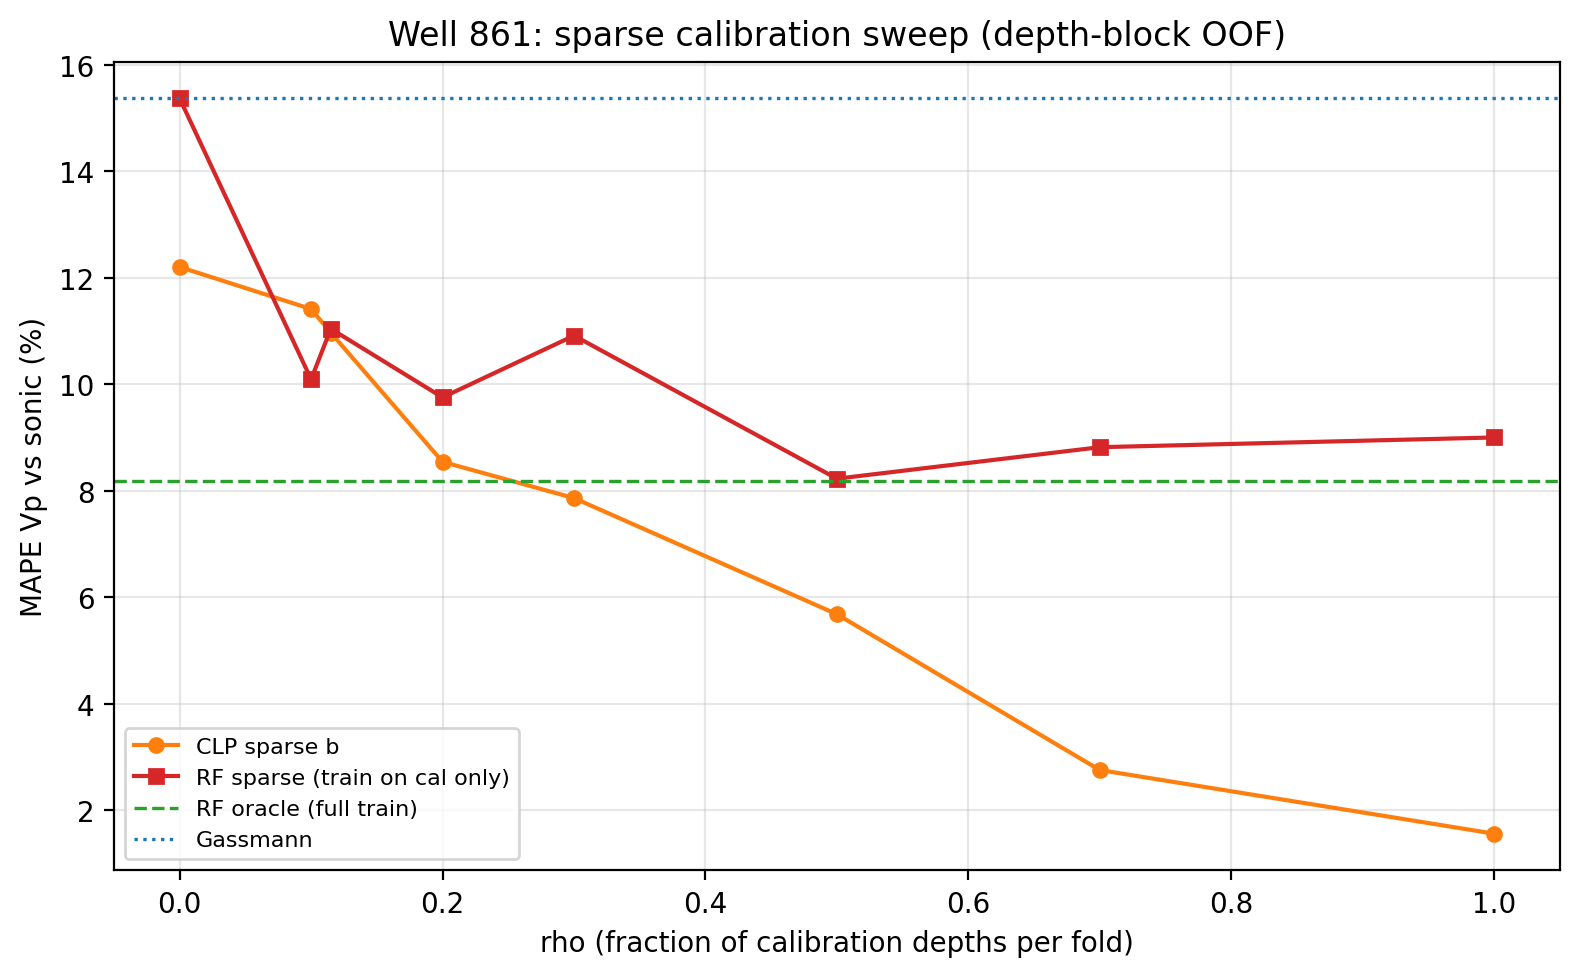
\includegraphics[width=0.85\linewidth]{figures/fig3_rho_sweep_mape}
  \caption{MAPE versus $\rho$: CLP sparse $b$ versus RF sparse. Linhas de
           referência: RF oracle (treino completo, tracejado verde) e Gassmann
           (pontilhado azul). O CLP cruza
           o oracle em $\rho \approx 0{,}7$; com dez plugs ($\rho \approx 0{,}12$)
           permanece no patamar $\approx 6{,}5\%$, próximo do baseline físico.}
  \label{fig:rho_sweep}
\end{figure}

\textbf{Leitura operacional:}
\begin{itemize}
  \item Há sônico denso no treino do residual?
        $\rightarrow$ mantenha o RF pontual (oracle).
  \item Caso contrário, a decisão depende de $\rho$:
        para $\rho\lesssim 0{,}5$, CLP e RF esparso empatam perto do
        Gassmann (pouca correção útil);
        para $\rho\gtrsim 0{,}7$, o CLP cruza o oracle---exigência alta
        e pouco realista em poço novo.
\end{itemize}
Sem sônico denso no treino, o CLP só compensa a
partir de calibração esparsa em $\gtrsim 70\%$ das profundidades; com apenas
dez plugs, RF sparse e CLP são ambos próximos do Gassmann e muito
inferiores ao RF oracle.
A mensagem prática é que a densidade de calibração, não o algoritmo, é o
fator limitante nesse regime.

\subsection{Síntese das Etapas~1--3}
\label{sec:sintese}

A Tabela~\ref{tab:project_summary} reúne, em um unico lugar, os patamares
obtidos nas três etapas do poço~861 (rodada junho de 2026).
Deve ser lida como mapa de continuidade: a Etapa~1 define o que o perfil
consegue prever e o protocolo de validação; a Etapa~2 entrega \Vp{}
física calibrada e documenta o viés residual frente ao DSI; a Etapa~3
ataca esse viés sem abandonar DEM/SC.

\begin{table}[H]
  \centering
  \caption{Síntese do projeto \emph{methods\_comparison} no poço~861:
           pergunta, escala de validação e métrica-chave por etapa.
           \emph{Nota:} métricas elásticas (linhas 5--8) referem-se ao
           mesmo poço (junho de 2026); validação intra-poço.}
  \label{tab:project_summary}
  \small
  \begin{tabular}{p{1.4cm}p{3.6cm}p{2.8cm}p{2.2cm}p{1.6cm}c}
    \toprule
    Etapa & Pergunta central & Validação & Métrica-chave & Valor & $n$ \\
    \midrule
    1 & \philab{} prevível com perfil? & depth-block OOF & $R^2$ (RF) & 0,15 & 87 \\
    1 & \fzilab{} prevível com perfil? & depth-block OOF & $R^2$ (RF) & $-0{,}82$ & 87 \\
    2 & \Vp{} DEM fecha laboratório? & LOO plugs & MAPE (\%) & 14,8 & 10 \\
    2 & \Vp{} Gassmann fecha DSI? & casamento 87/87 & MAPE (\%) & 7,3 & 87 \\
    2 & Gassmann reduz viés vs seco? & casamento 87/87 & Viés (km/s) & $+0{,}27$ & 87 \\
    3 & Resíduo prevível com perfil? & depth-block OOF & $R^2$ resíduo & 0,79 & 87 \\
    3 & Híbrido fecha DSI? & depth-block OOF & MAPE (\%) & 2,8 & 87 \\
    3 & Híbrido elimina viés? & depth-block OOF & Viés (km/s) & $+0{,}01$ & 87 \\
    3b & CLP residual fecha DSI? & depth-block OOF & MAPE (\%) & 6,3 & 87 \\
    3b & CLP vs RF (melhor CLP) & depth-block OOF & $\Delta$MAPE (pp) & $+3{,}6$ & 87 \\
    \bottomrule
  \end{tabular}
\end{table}

Na Tabela~\ref{tab:project_summary}, a progressão entre etapas é explícita.
A Etapa~1 estabelece que porosidade é viável ($R^2 \approx 0{,}15$) e que FZI
direto de perfil falha ($R^2 \approx -0{,}82$), orientando a Etapa~2 para DEM/SC
com \phiND{} e HFU de laboratório em vez de ML perfil $\rightarrow$ \Vp{}.
A Etapa~2 confirma viabilidade física no laboratório (LOO $\approx 15\%$ MAPE),
mas deixa viés $+0{,}27$~km/s no DSI mesmo após Gassmann---linha que motiva
a Etapa~3.
O híbrido OOF reduz MAPE de \Vp{} para 2,8\% e viés para $+0{,}01$~km/s,
fechando parcialmente o \emph{gap} identificado na síntese da Etapa~2.
Vale contrastar as duas linhas de validação da Etapa~2: o LOO de plugs
(14,8\%, $n=10$) é bem pior que o casamento com o perfil (7,3\%, $n=87$),
porque cada plug retirado remove uma fração grande da informação de
calibração da sua HFU---o perfil, ao contrário, é avaliado com todos os plugs
dentro do ajuste.
Os resultados demonstram \textbf{consistência local no poço~861} e indicam
\emph{potencial} de generalização; validação interpoços permanece
necessária.
Nenhuma linha da tabela substitui as outras: cada etapa responde a uma pergunta
distinta na cadeia perfil $\rightarrow$ física $\rightarrow$ correção residual.

\section{Discussão}
\label{sec:discussao}

\subsection{Papel do ML na cadeia física}

O híbrido demonstra que \emph{parte substancial} do viés pós-Gassmann
é explicável por padrões nas curvas de perfil, condicionados à baseline
física.
Geologicamente, isso é compatível com heterogeneidade de facies carbonática,
variação de argilosidade e limitações do PVT default ($K_f$ de
formação, saturação total assumida) que o DEM/SC por HFU não resolve
linha a linha.
O ML atua como \textbf{corretor empírico local}---análogo, em espírito, ao
RF de \philab{} na Etapa~1, mas aplicado ao resíduo elástico em vez da
porosidade direta.
O corretor melhora o ajuste frente ao DSI, porém \textbf{não identifica uma
única causa física}: o resíduo modelado pode combinar pressão efetiva,
limitações de Gassmann e PVT default, erro de segmentação HFU,
anisotropia, mineralogia residual, condição de medida do DSI (frequência,
escala de investigação) e imperfeições do DEM/SC calibrado.
Não deve ser interpretado como novo modelo físico nem como explicação
mecanística única do desvio elástico.

Importante: o ganho não invalida a Etapa~2.
Sem Gassmann, o viés contra o sônico era similar; sem DEM/SC calibrado, não
haveria baseline interpretável para inversão.
A Etapa~3 fecha um \emph{gap operacional} identificado na própria discussão
da Etapa~2, não propõe substituir a física por caixa-preta.

\subsection{Hipótese de porosidade (\phiND{}) e composição do residual}
\label{sec:phi_nd_hypothesis}

A escolha de \phiND{} como porosidade de entrada na Etapa~2---e, portanto,
na tendência física fixa da Etapa~3---não é metodologicamente errada; é
defensável, desde que a hipótese seja explícita.
A mesma \phiND{} desempenha dois papéis físicos distintos.

No DEM, a porosidade controla quanto o espaço poroso reduz a rigidez da
matriz mineral:
\begin{equation}
  (K_m,G_m)
  \xrightarrow[\alpha]{\phiND{}}
  (K_{\mathrm{dry}},G_{\mathrm{dry}}).
\end{equation}
Mesmo poros que pouco contribuem para o escoamento podem deformar e
amolecer o arcabouço; para o meio seco, uma estimativa de porosidade
\emph{total} de perfil é, portanto, razoável.

Em Gassmann, a hipótese é mais restritiva: o formalismo pressupõe
comunicação hidráulica e equilíbrio de pressão do fluido no espaço poroso.
A porosidade teoricamente relevante é a parcela conectada que participa da
pressurização.
Ao reutilizar \phiND{} na saturação, o modelo de \textbf{porosidade única}
adota aproximadamente
\begin{equation}
  \phi_{\mathrm{mecanica}}
  \approx
  \phi_{\mathrm{hidraulicamente\ ativa}}
  \approx
  \phiND{}.
\end{equation}
Essa aproximação é comum e mais defensável em carbonato relativamente
limpo, com baixa fração de argila; pode degradar-se na presença de vugs
isolados ou poros que não entram no equilíbrio de pressão.
Não afirmamos que \phiND{} seja porosidade efetiva (PHIE) medida: ela é a
estimativa contínua disponível de porosidade total, usada de forma
\textbf{consistente} no DEM e em Gassmann.

A formulação da Etapa~3 permanece
\begin{equation}
  V_{\mathrm{p,sonic}}
  =
  V_{\mathrm{p,Gassmann}}(\phiND{},\mathrm{HFU},\theta)
  + g(X) + \varepsilon,
\end{equation}
com tendência física previamente fixada e
$g(X)\approx\mathbb{E}[\Delta V_{\mathrm{p}}\mid X]$
(Seção~\ref{sec:form_estat}).
Se \phiND{} não coincidir com a porosidade fisicamente mais apropriada,
parte do erro entra no residual
$\Delta V_{\mathrm{p}} = V_{\mathrm{p,sonic}} - V_{\mathrm{p,Gassmann}}$.
Em primeira ordem (Apêndice~\ref{app:phi_taylor}), isolando apenas $\phi$
com HFU e $\theta$ fixos ($F_\phi=\partial F/\partial\phi$),
\begin{equation}
  \label{eq:dvp_phi_taylor}
  \Delta V_{\mathrm{p}}
  \approx
  -F_\phi(\phiND{},\theta,h)\,\delta\phi
  + r_{\mathrm{outros}} + \varepsilon,
\end{equation}
onde $\delta\phi=\phiND{}-\phi^{*}$ e $r_{\mathrm{outros}}$ agrupa
diferenças físicas além de $\phi$: $S_w$, $K_f$, frequência
(Gassmann vs.\ sônico), pressão efetiva, anisotropia, mineralogia,
geometria porosa ($\alpha$), HFU mal atribuída, heterogeneidade abaixo
da resolução do perfil e interações entre esses mecanismos.
Com $\mathbb{E}[\varepsilon\mid X]=0$,
\begin{equation}
  g(X)
  \approx
  \mathbb{E}\bigl[-F_\phi\,\delta\phi + r_{\mathrm{outros}}\bigm| X\bigr]:
\end{equation}
o corretor \textbf{não} aprende $F_\phi$; aprende a contribuição
previsível dessa soma a partir de $X$.

\textbf{Conclusão cuidadosa sobre o sinal.}
Na faixa usada, $F_\phi<0$. Se $\delta\phi\ge 0$
($\phi^{*}$ efetiva menor que \phiND{}), o termo isolado
$-F_\phi\delta\phi\ge 0$ empurra $\Delta V_{\mathrm{p}}$ para cima.
Observamos o contrário:
$V_{\mathrm{p,Gassmann}}>V_{\mathrm{p,sonic}}$
$\Rightarrow$ $\Delta V_{\mathrm{p}}<0$
($\mu_\Delta\approx -0{,}27$~km/s).
Portanto uma porosidade efetiva menor \textbf{não pode ser a causa isolada}
do residual negativo---não implica $\delta\phi=0$ nem que \phiND{} esteja
``correta''; $\phi$ ainda pode participar do erro, mas com sinal
contrário ao viés total.
Em média,
$\mu_\Delta
\approx\mathbb{E}[-F_\phi\delta\phi]+\mathbb{E}[r_{\mathrm{outros}}]$;
como $\mu_\Delta<0$ e $\mathbb{E}[-F_\phi\delta\phi]\ge 0$ sob a hipótese
$\delta\phi\ge 0$, necessariamente $\mathbb{E}[r_{\mathrm{outros}}]<0$
(os demais mecanismos devem dominar o sinal).
Exemplo numérico: $-F_\phi\delta\phi=+0{,}10$ e
$r_{\mathrm{outros}}=-0{,}40$ já produzem
$\Delta V_{\mathrm{p}}\approx -0{,}30$~km/s.

Seria problemático: (i)~chamar \phiND{} de PHIE medida; (ii)~trocar a
porosidade na Etapa~3 sem recalcular DEM, Gassmann e o residual;
(iii)~afirmar que o corretor isolou o mecanismo do desvio;
(iv)~declarar transferência automática para outro poço;
(v)~afirmar simplesmente que ``a escolha de \phiND{} não explica o viés''
sem a ressalva de causa \emph{isolada}.
A coerência Etapa~2~$\rightarrow$~Etapa~3 exige manter a mesma \phiND{} na
baseline física.

\subsection{CLP-CSGM versus regressão pontual}

A Etapa~3b (Seção~\ref{sec:clp_vp_residual}) testou reconstrução CLP-CSGM
em janelas sobre o mesmo resíduo.
O melhor CLP (plug sparse $b$, 6,3\% MAPE) ficou $\approx 3{,}6$ pontos
percentuais acima do RF (2,8\%), coerente com a escala fina do resíduo
e com a disponibilidade do sônico em todo o intervalo como alvo de treino.
O sweep $\rho$ (Seção~\ref{sec:rho_sweep}) quantifica a condição de virada:
o CLP só supera o oracle com calibração esparsa acima de $\approx 70\%$ das
profundidades, o que restringe bastante o cenário em que ele compensa.
O CLP permanece relevante para cenários com \textbf{medidas esparsas} em $b$
(análogo à Etapa~1f); para correção residual em perfil completo, o RF
pontual é superior neste poço.

\subsection{Sensibilidade ao fluido ($K_f$, $S_w$)}
\label{sec:kf_sensitivity}

O produto oficial mantém fluido \textbf{constante} no Gassmann:
$S_w=1$, $K_f=2{,}2$~GPa e $\rho_f=1{,}03$~g/cc (água de formação, PVT
default da Etapa~2b).
No intervalo modelado (5205,9--5233,7~m), a curva LAS confirma
$S_w=1$ ponto a ponto, e a curva \texttt{KFluid} do processamento
petrofísico/PVT tem mediana $\approx 2{,}83$~GPa com variação pequena em
profundidade (Figura~\ref{fig:kf_sw_las}).
Isso motiva um teste A/B controlado: mesmo DEM seco, mesma \phiND{},
mesma HFU e mesmos blocos OOF; só o fluido ($K_f$, $\rho_f$) muda no
Gassmann, e o híbrido é re-treinado em OOF.

\begin{figure}[H]
  \centering
  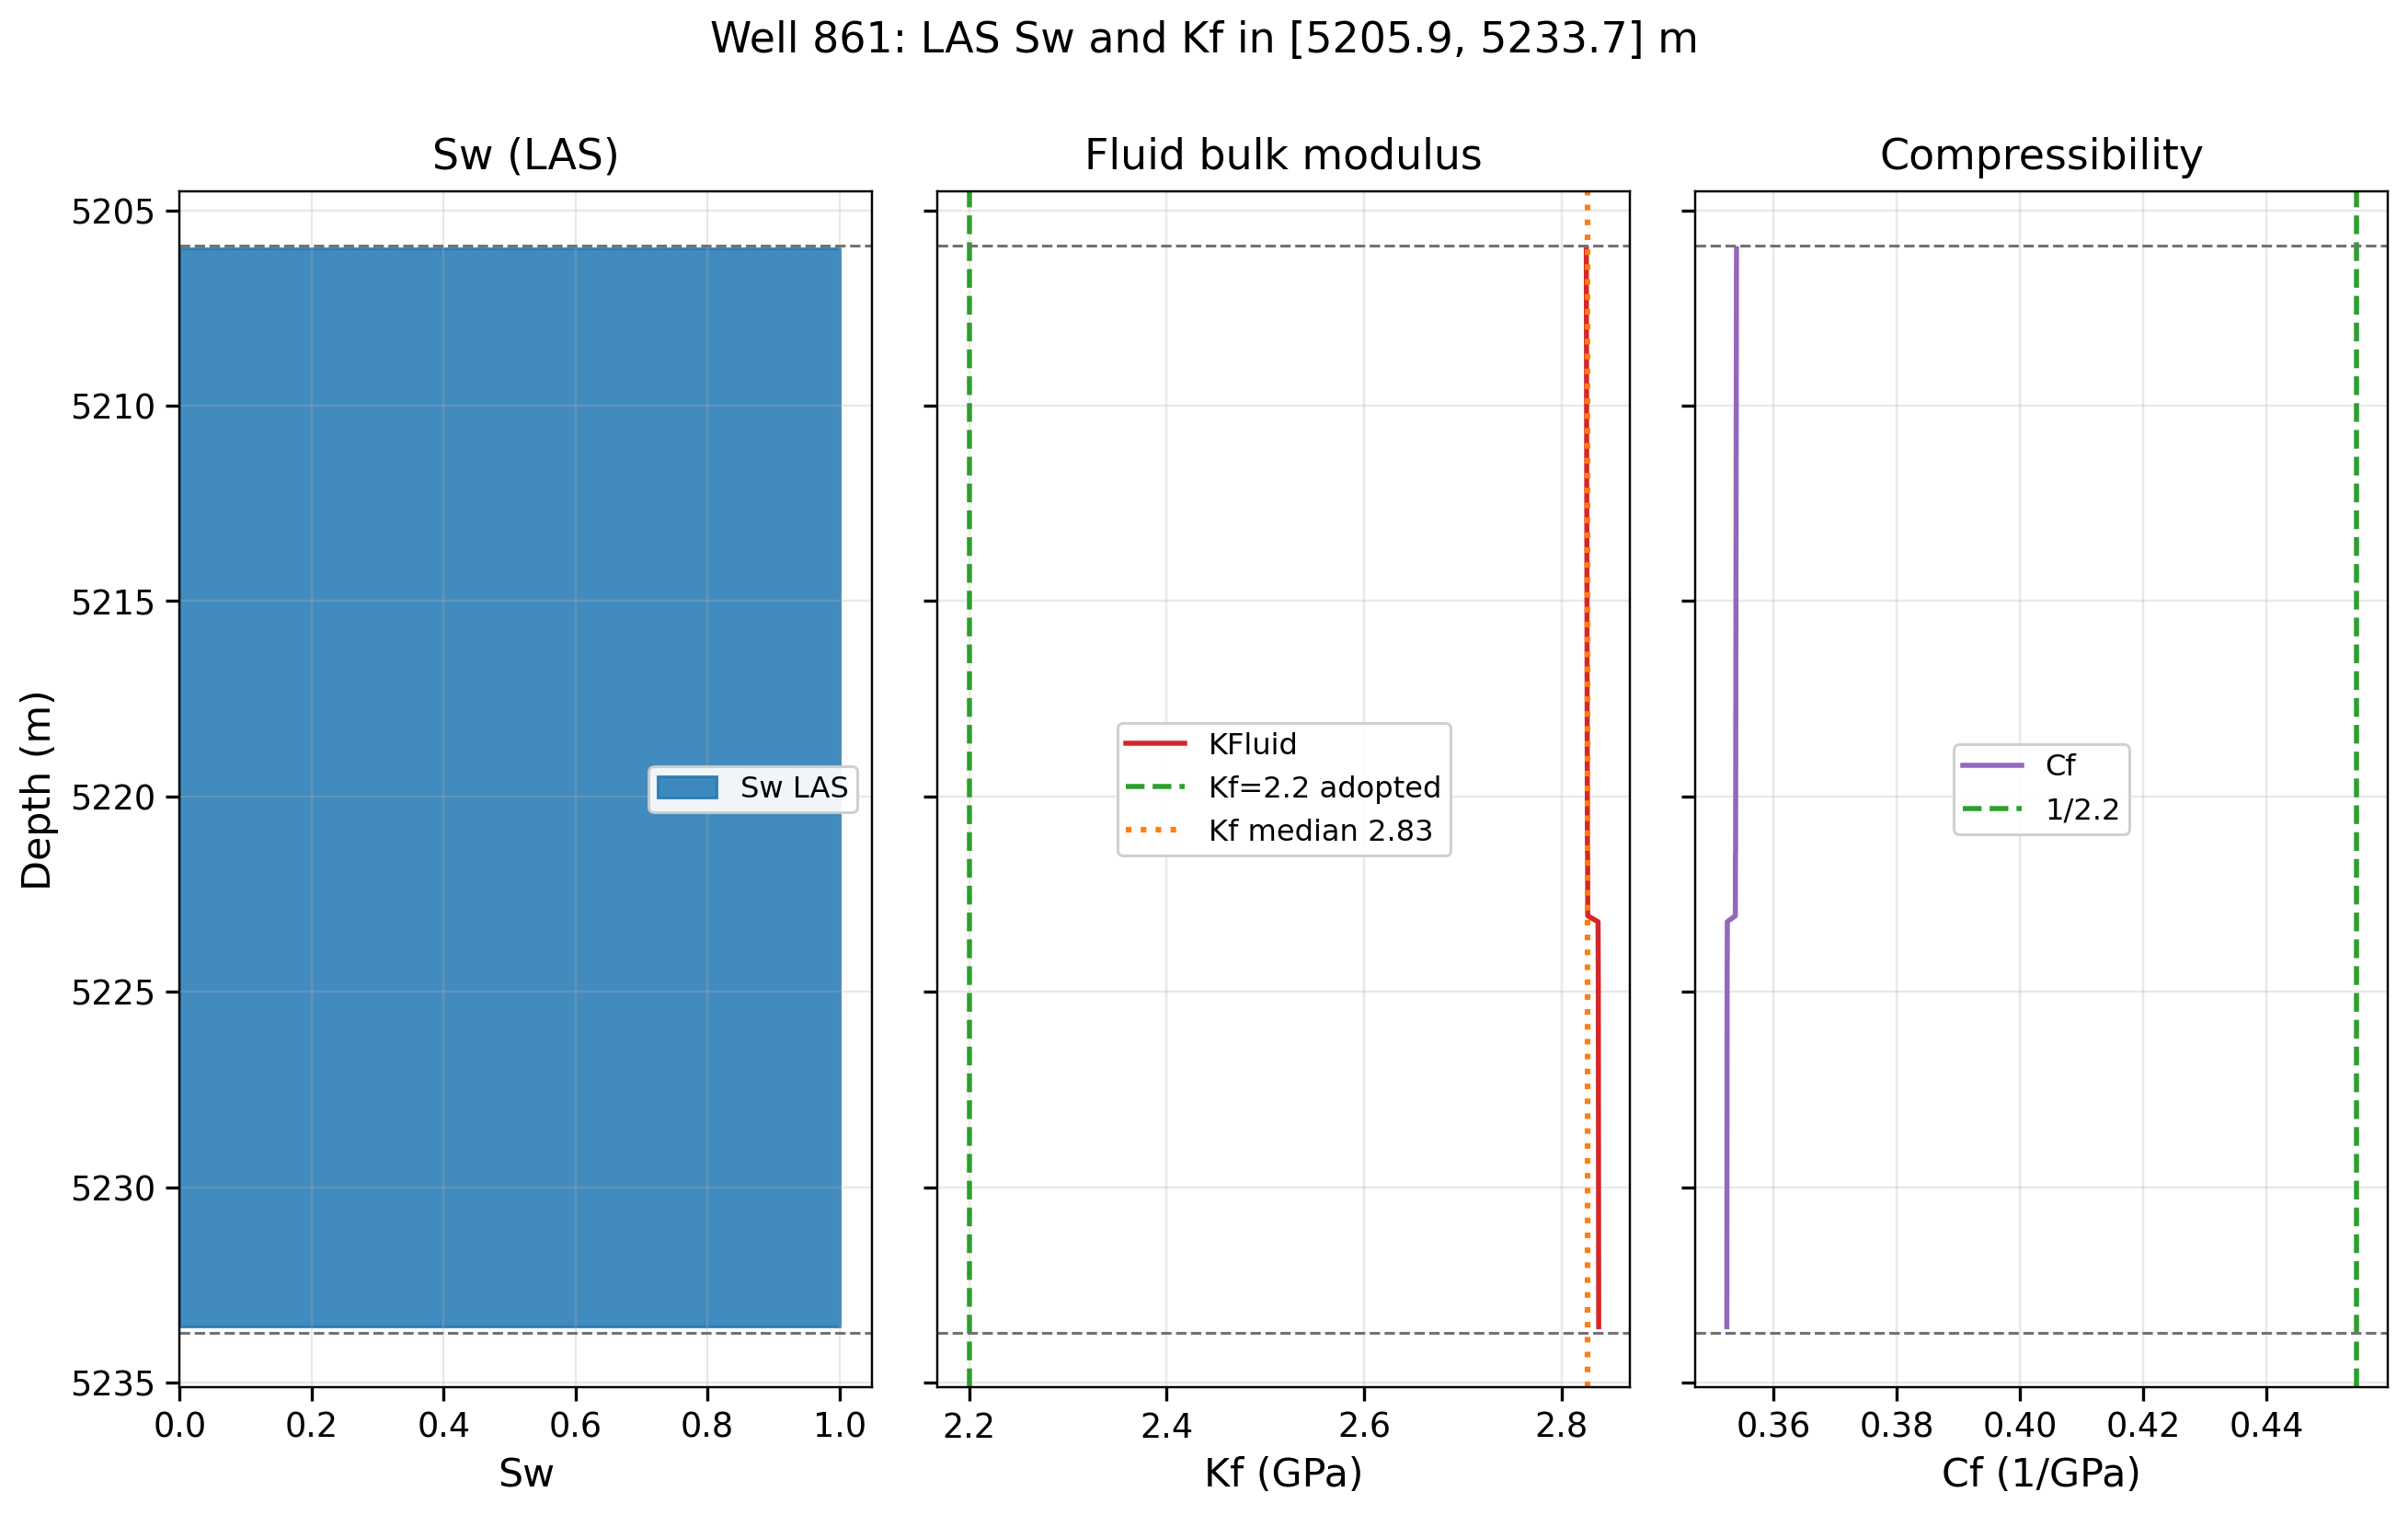
\includegraphics[width=0.92\linewidth]{figures/fig3_kf_sw_study_interval}
  \caption{Intervalo do modelo: $S_w$ (LAS), $K_f$ (\texttt{KFluid}) e
  $C_f=1/K_f$. Verde: $K_f=2{,}2$~GPa adotado; laranja: mediana do perfil.}
  \label{fig:kf_sw_las}
\end{figure}

A Tabela~\ref{tab:kf_sensitivity} resume o default, a mediana de poço
e o cenário NMR VRH (perfil $K_f(z)$).
Atualizar o default para a mediana de poço ($\approx 2{,}83$~GPa) quase não
altera o MAPE Gassmann (7,28\% em ambos) e deixa o híbrido RF praticamente
igual (2,78\% $\rightarrow$ 2,81\%, $+0{,}03$~p.p.); a linear permanece em 2,10\%.
O viés Gassmann sobe ligeiramente ($+0{,}271 \rightarrow +0{,}295$~km/s):
$K_f$ menor (2,2~GPa) deixa o fluido um pouco mais compressível e o
$V_{\mathrm{p}}$ um pouco mais baixo, o que \emph{compensa} parcialmente o
viés positivo---efeito de nível, não de fluido ``mais certo''.

Como cenário NMR, misturamos água e óleo via \texttt{SWIRR} com a média
de Voigt--Reuss--Hill (VRH). Não é correção física da mistura iso-tensão
nem modelo de saturação heterogênea/patchy:
\begin{equation}
  \label{eq:kf_vrh}
  K_V = S_w K_{\mathrm{brine}} + S_o K_{\mathrm{oil}},
  \qquad
  \frac{1}{K_R}
  =
  \frac{S_w}{K_{\mathrm{brine}}}
  +
  \frac{S_o}{K_{\mathrm{oil}}},
  \qquad
  K_{\mathrm{VRH}} = \frac{K_V + K_R}{2}.
\end{equation}
A densidade é volumétrica,
$\rho_f = S_w\rho_{\mathrm{brine}}+S_o\rho_{\mathrm{oil}}$.
Após a mistura, o Gassmann é chamado com $S_w=1$: $K_f$ e $\rho_f$ já
representam o fluido que ocupa o poro; passar \texttt{SWIRR} de novo
multiplicaria indevidamente a densidade.
No intervalo, a mediana de $S_w^{\mathrm{NMR}}$ (após recorte) é
$\approx 0{,}31$ ($S_o\approx 0{,}69$), $K_f$ VRH $\approx 1{,}40$~GPa
e $\rho_f\approx 0{,}80$~g/cc (Figura~\ref{fig:kf_sw_nmr}).
Três amostras LAS/rock no intervalo têm \texttt{SWIRR}$<0$
(5205,984; 5206,136; 5206,289~m) e foram recortadas para $0$;
duas entram nas 87 linhas do modelo.
Esse recorte é bound numérico, não evidência de óleo puro.
\texttt{SWIRR} permanece proxy de saturação irredutível, não $S_w$ in situ.
A porosidade de entrada permanece \phiND{}: papéis distintos
($\phi$ = volume de poro; $S_w$ = preenchimento).

\begin{figure}[H]
  \centering
  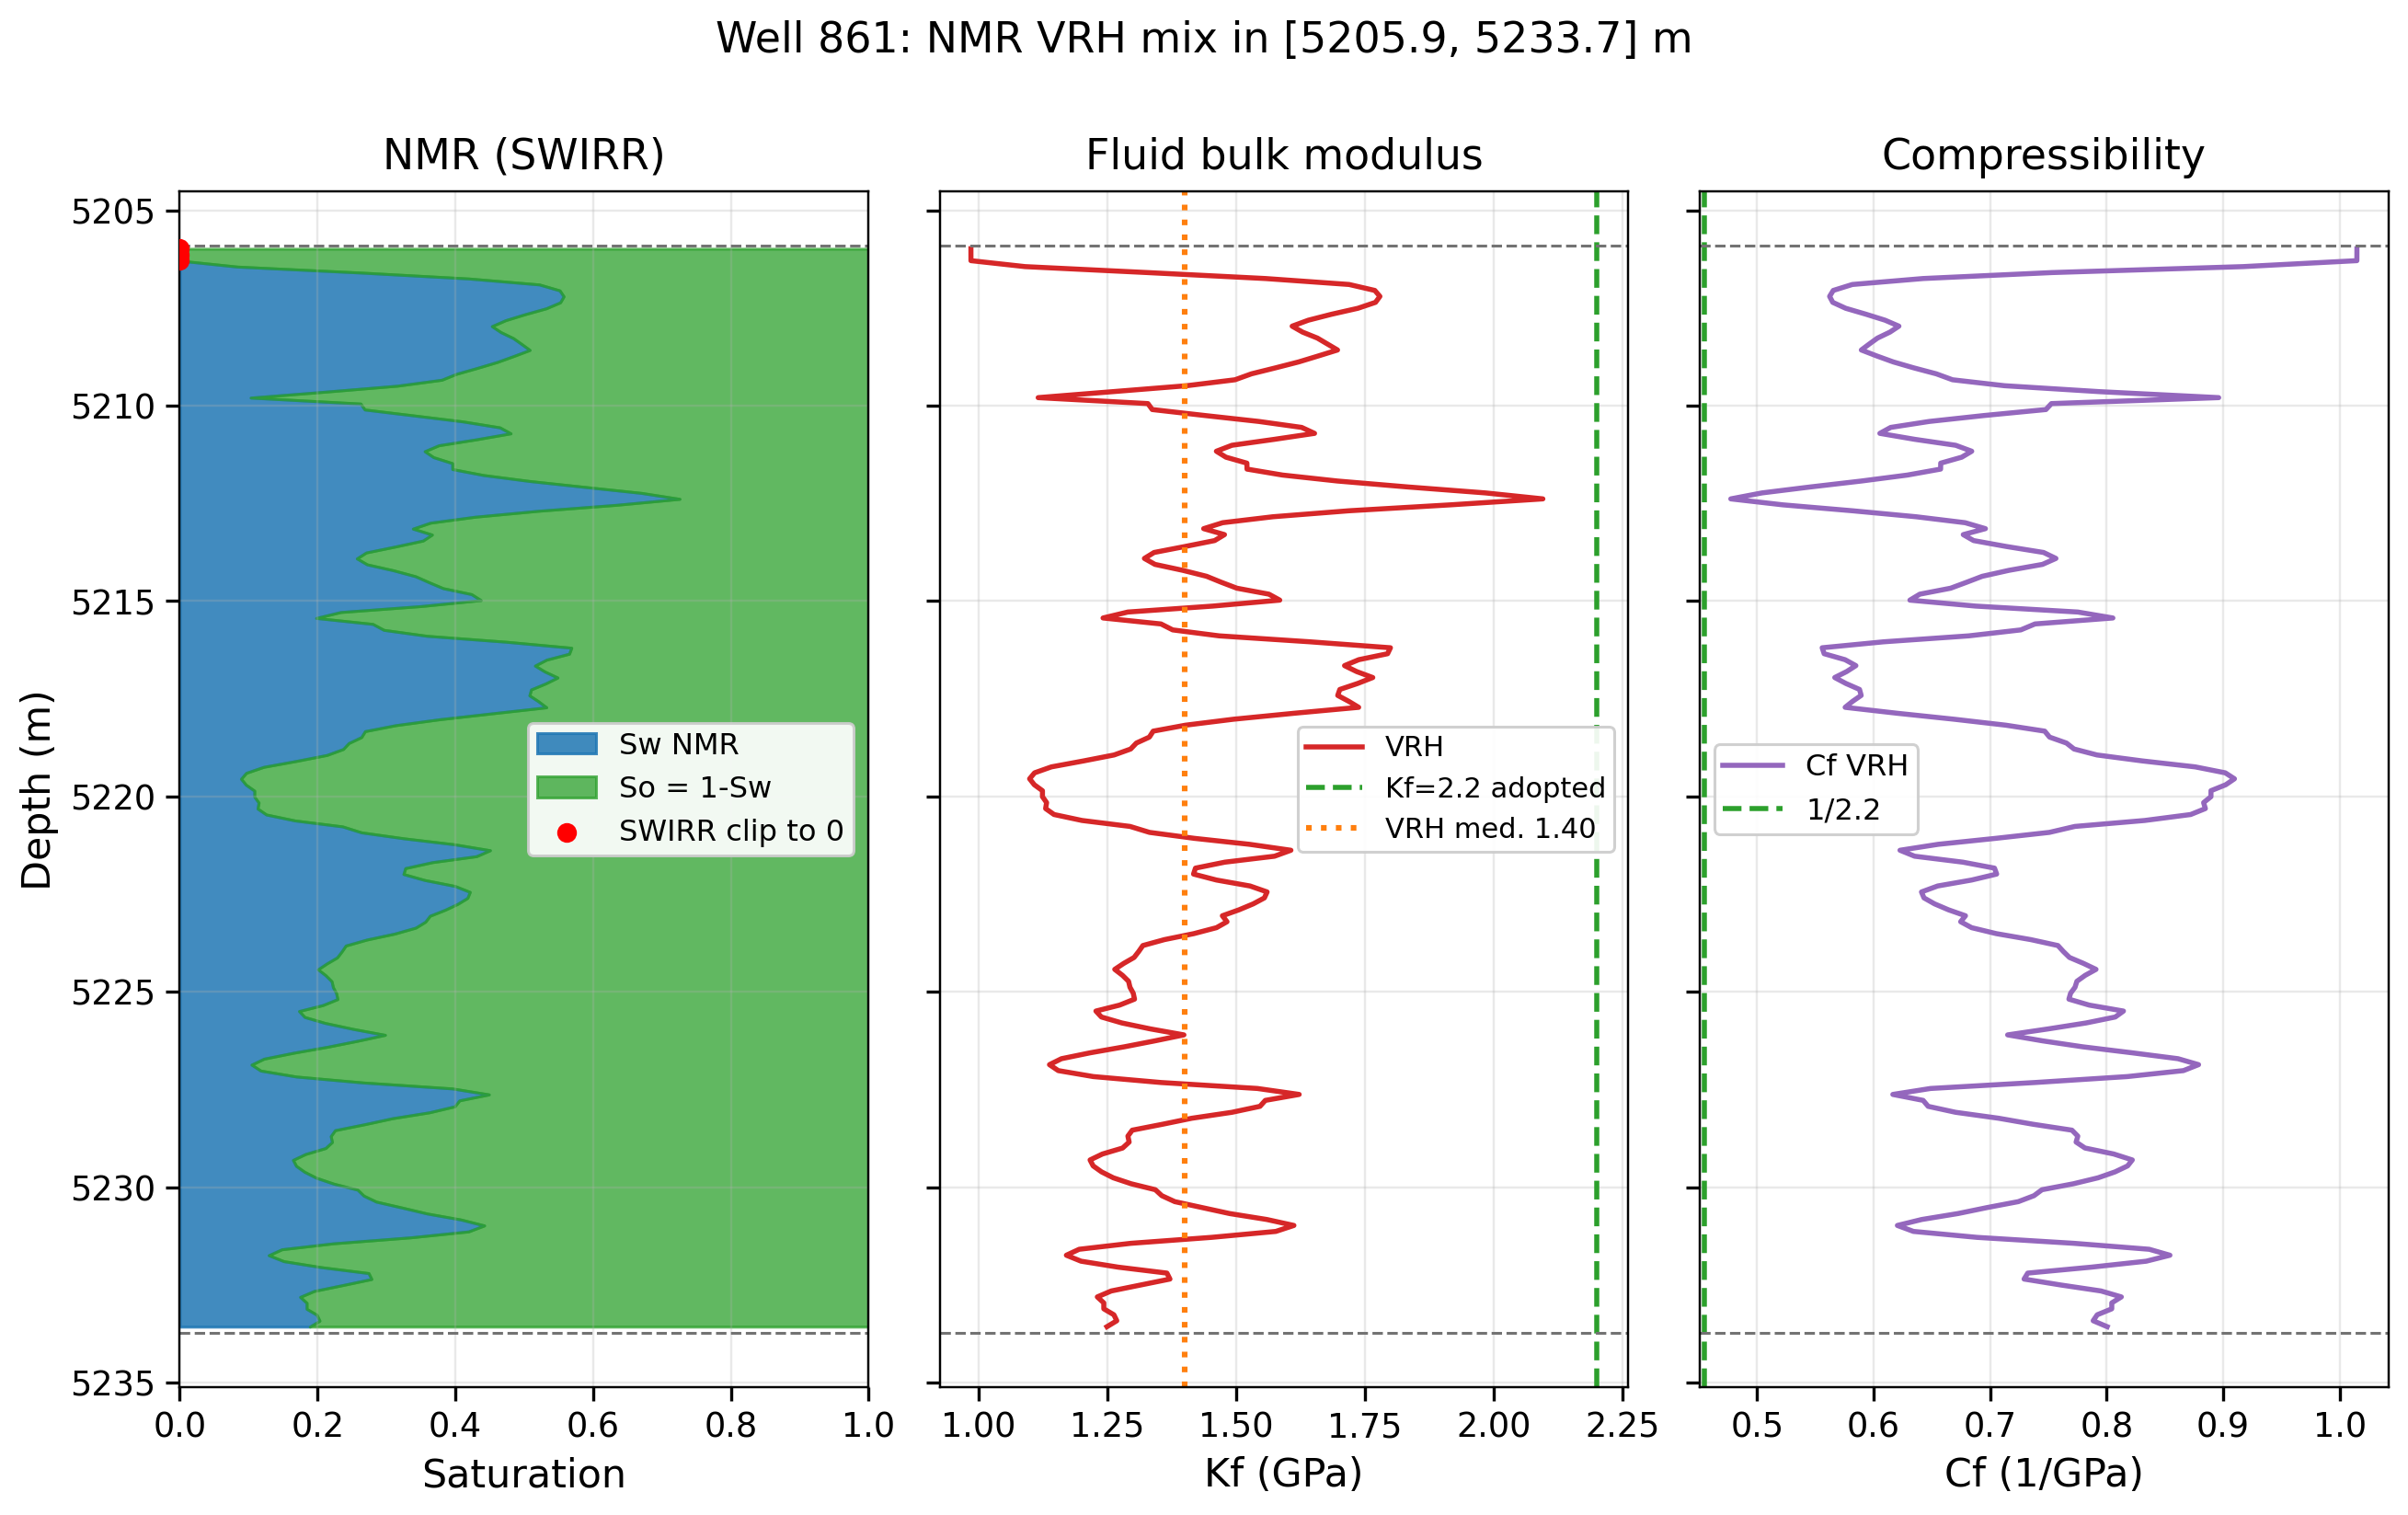
\includegraphics[width=\linewidth]{figures/fig3_kf_sw_nmr_study_interval}
  \caption{Alternativa NMR com mistura VRH: $S_w$/\texttt{SWIRR}
  (recortes em vermelho), $K_f$ VRH e $C_f=1/K_f$.
  Verde: $K_f=2{,}2$~GPa adotado; laranja: mediana VRH
  ($\approx 1{,}40$~GPa).}
  \label{fig:kf_sw_nmr}
\end{figure}

\begin{table}[H]
  \centering
  \caption{MAPE (\%) e viés (km/s) no intervalo modelado
  (87 linhas, OOF em 3~blocos).
  As três colunas compartilham o DEM seco e a \phiND{};
  só o fluido no Gassmann muda. NMR = mistura VRH no perfil $K_f(z)$.}
  \label{tab:kf_sensitivity}
  \scriptsize
  \setlength{\tabcolsep}{4pt}
  \begin{tabular}{lcccccc}
    \toprule
    & \multicolumn{2}{c}{$K_f=2{,}2$} &
      \multicolumn{2}{c}{$K_f\approx 2{,}83$} &
      \multicolumn{2}{c}{VRH NMR} \\
    \cmidrule(lr){2-3}\cmidrule(lr){4-5}\cmidrule(lr){6-7}
    Etapa & MAPE & Viés & MAPE & Viés & MAPE & Viés \\
    \midrule
    Gassmann & 7,28 & $+0{,}271$ & 7,28 & $+0{,}295$ &
      7,63 & $+0{,}266$ \\
    Híbr.\ RF & 2,78 & $+0{,}014$ & 2,81 & $+0{,}017$ &
      2,91 & $+0{,}016$ \\
    Híbr.\ lin. & 2,10 & $+0{,}002$ & 2,10 & $+0{,}002$ &
      2,10 & $+0{,}002$ \\
    \bottomrule
  \end{tabular}
\end{table}

VRH piora um pouco o MAPE frente ao adotado (Gassmann
$\approx +0{,}35$~p.p.; RF $\approx +0{,}14$~p.p.); a linear fica igual.
Perfil $K_f(z)$ e mediana VRH produzem métricas \emph{próximas, não iguais}
(7,63\% vs 7,62\%).
Isso não demonstra que $K_f$ varie pouco
(VRH $\approx 1{,}0$--$2{,}1$~GPa neste intervalo):
o produto (MAPE/viés) é pouco sensível a usar o perfil ou a mediana.
\textbf{Decisão:} mantemos $K_f=2{,}2$~GPa no fluxo oficial; mediana de
poço e VRH+\texttt{SWIRR} ficam como testes de sensibilidade.
O script \texttt{run\_861\_kf\_fluid\_sensitivity.py} regenera figuras e
tabelas sob
\texttt{methods\_comparison/results/kf\_fluid\_sensitivity\_861/}.

\subsection{Limitações metodológicas}

Cinco limitações devem acompanhar qualquer uso dos números desta etapa.
\textbf{(i)} Amostra pequena (87 linhas, oito \emph{features}): complexidade do
modelo foi mantida modesta (RF com 200 árvores) para reduzir risco de
sobreajuste; mesmo assim, HFU~4 com $n=6$ permanece estatisticamente frágil,
e é justamente ela que concentra o maior ganho reportado.
\textbf{(ii)} Validação OOF no \emph{mesmo poço}: blocos de profundidade
evitam vazamento espacial trivial, mas o sônico entra no alvo residual---a
OOF não equivale a poço ou intervalo independente; extrapolação fora
de campo Lapa não está demonstrada.
\textbf{(iii)} Fluido no Gassmann: o produto usa PVT fixo
($K_f=2{,}2$~GPa, $S_w=1$, $\rho_f=1{,}03$~g/cc).
A Seção~\ref{sec:kf_sensitivity} explorou a mediana de poço
($\approx 2{,}83$~GPa) e VRH+\texttt{SWIRR} (figura NMR).
Nenhuma melhorou o produto frente ao sônico neste intervalo, mas pressão efetiva e
outras condições in situ continuam fora do escopo.
\textbf{(iv)} O MAPE de 2,8\% é baixo em termos absolutos, mas mede
interpolação em profundidade dentro de um intervalo de 28~m com amostragem
densa; blocos vizinhos compartilham facies, de modo que o teste é menos severo
do que a rotulação ``fora-da-amostra'' pode sugerir.
\textbf{(v)} Hipótese de porosidade única (\phiND{} no DEM e em Gassmann):
diferenças entre porosidade total e hidraulicamente ativa fazem parte da
incerteza da tendência física e podem contribuir para $\Delta V_{\mathrm{p}}$
(Seção~\ref{sec:phi_nd_hypothesis}); a física não foi reajustada com o sônico.

\subsection{Random Forest versus alternativas e próximos passos}
\label{sec:proximos_passos}

A Tabela~\ref{tab:regressor_sensitivity} mostra que a regressão linear
entregaria MAPE ainda menor que o RF (2,1\% versus 2,8\%), com viés
igualmente desprezível.
Isso é um argumento a favor da simplicidade: se o resíduo é aproximadamente
linear nas curvas e na baseline física, um corretor linear é mais fácil de
auditar, exportar e transferir para outro poço do que um ensemble.
Mantemos o RF no produto documentado por alinhamento à Etapa~1; testes futuros
podem exportar ambas as trilhas e comparar estabilidade interpoços, onde a
vantagem do modelo mais simples tende a crescer.

\textbf{Decisão operacional no poço~861.}
Só física (Gassmann) basta onde a HFU~2 já fecha ($\mathrm{MAPE}\approx 2\%$),
quando não há sônico denso para treinar o residual, ou quando a
interpretabilidade da cadeia DEM--Gassmann é prioritária.
O híbrido RF é preferível no mesmo poço com sônico no alvo---em especial
HFU~3/4---e convém reportar também a trilha linear (sensibilidade).

\textbf{Testes A/B no poço \#1045 (próximo passo de generalização).}
\begin{itemize}
  \item \textbf{Teste~A (transferir o corretor):}
        treina Gassmann $+$ residual no 861; aplica em \#1045 com
        perfis e Gassmann \emph{local}; o sônico do 1045 entra
        \textbf{só} na avaliação---o modelo \textbf{não} é retreinado
        no sônico do poço novo.
  \item \textbf{Teste~B (reproduzir o método):}
        Gassmann local no poço novo + aprendizado residual em blocos
        de profundidade do próprio \#1045 (sônico no alvo, como aqui).
\end{itemize}
Nos dois testes: Gassmann local; \phiS{} e $\Delta t$ fora de $X$.
Só após A/B faz sentido exportar o híbrido a perfil de produção /
inversão sísmica.
Para produção de perfil no 861, o próximo passo natural permanece exportar
a coluna $V_{\mathrm{p,hybrid}}$ (RF ou regressão linear) ao produto
integrado e repetir a validação tripla da Etapa~2 (laboratório onde houver
plugs, \phiND{} versus \phiS{}, DSI) com a nova trilha.
Recomenda-se também refinamento de PVT onde houver amostras de fluido
(a Seção~\ref{sec:kf_sensitivity} já quantifica que mediana de poço e
VRH+\texttt{SWIRR} não melhoram o produto neste intervalo).

\section{Conclusões}
\label{sec:conclusoes}

\begin{enumerate}
  \item \textbf{Viabilidade do híbrido:} no poço~861, ML sobre resíduos
        pós-Gassmann reduz MAPE de \Vp{} de 7,3\% para 2,8\% e viés de
        $+0{,}27$ para $+0{,}01$~km/s no OOF, alinhando a média predita ao
        patamar sônico; parte do desvio DEM/Gassmann--DSI é modelável por
        variáveis de perfil em escala local.
  \item \textbf{Papel na cadeia:} o ML é \textbf{corretor empírico} da física
        DEM/SC + Gassmann, não substituto do sônico nem atalho perfil
        $\rightarrow$ \Vp{}; não constitui novo modelo físico.
  \item \textbf{HFU:} maior ganho em HFU~4 (sem plugs,
        MAPE $\approx 28\% \rightarrow 5\%$ no OOF, $n=6$) e HFU~3
        ($11{,}5\% \rightarrow 5{,}4\%$); a HFU~2 já era boa
        ($\approx 2\%$) e permanece estável, sem ganho nem degradação---o
        corretor compensa deficiência de calibração, não física ausente.
  \item \textbf{Validação:} depth-block OOF é honesta em profundidade no
        poço~861, mas o sônico entra no alvo---não equivale a poço cego;
        generalização interpoços permanece hipótese a testar.
  \item \textbf{\phiS{}:} excluída de $X$ por ser transformada de Wyllie do
        DTCO que define o alvo ($r = -0{,}993$ com $V_{\mathrm{p,sonic}}$);
        admiti-la inflaria o MAPE aparente em $\approx 0{,}6$ ponto percentual
        sem ganho preditivo real.
  \item \textbf{Regressor:} RF oficial (MAPE 2,8\%, viés $+0{,}01$); regressão
        linear ainda melhor (2,1\%), GB e XGB próximos (3,0--3,6\%), Ridge sem
        padronização e MLP piores (6,1--6,5\%); o resultado não depende de um
        algoritmo específico.
  \item \textbf{CLP-CSGM:} as variantes por janelas (6,3--6,7\% MAPE) ficam
        atrás do RF pontual e só superam o oracle com calibração esparsa em
        $\gtrsim 70\%$ das profundidades.
  \item \textbf{Porosidade:} \phiND{} é entrada total de perfil (modelo de
        porosidade única), não PHIE medida; eventuais discrepâncias com a
        porosidade hidraulicamente ativa entram na incerteza da tendência e
        no residual (Seção~\ref{sec:phi_nd_hypothesis}).
        Isoladamente, $\phi^{*}$ menor que \phiND{} produz contribuição
        \textbf{positiva} a $\Delta V_{\mathrm{p}}$, oposta ao viés
        observado ($\Delta V_{\mathrm{p}}<0$); outros mecanismos
        ($r_{\mathrm{outros}}$) precisam dominar o sinal em média.
  \item \textbf{Fluido:} $K_f=2{,}2$~GPa ($S_w=1$) permanece no produto;
        mediana de poço ($\approx 2{,}83$~GPa) e VRH+\texttt{SWIRR}
        ($\approx 1{,}40$~GPa) não melhoram Gassmann nem o híbrido
        OOF frente ao sônico neste intervalo
        (Seção~\ref{sec:kf_sensitivity}).
  \item \textbf{Próximo passo:} exportar $V_{\mathrm{p,hybrid}}$ (RF ou
        regressão linear) ao perfil de produção; testes A/B no poço \#1045
        (transferir o corretor do 861 vs.\ reproduzir o método localmente)
        antes de inversão sísmica.
\end{enumerate}

\section*{Reprodutibilidade}

Os pipelines da Etapa~3 estão automatizados no repositório
\emph{methods\_comparison}.
A sequência dependente é: validação Gassmann (Etapa~2b), em seguida
aprendizado residual com validação por blocos de profundidade.
Artefatos exportados incluem tabelas de dataset, predições OOF, comparação
física versus híbrido, sensibilidade aos seis regressores
(\texttt{regressor\_sensitivity.csv},
\texttt{regressor\_oof\_vp\_depth.csv}), figuras de profundidade (RF e comparativa
por regressor) e \emph{scatter} do resíduo, modelo Random Forest serializado e manifesto com métricas da
rodada de junho de 2026.
A sensibilidade a fluido ($K_f$, $S_w$, VRH+\texttt{SWIRR}) é regenerada por
\texttt{scripts/run\_861\_kf\_fluid\_sensitivity.py}, com métricas, recortes de
\texttt{SWIRR} e manifesto em
\texttt{results/kf\_fluid\_sensitivity\_861/} e figuras
\texttt{latex/figures/fig3\_kf\_sw\_*.png}
(flag \texttt{--write-latex-figures}; conferência \texttt{--check-slides}
usa os mesmos arredondamentos da Tabela~\ref{tab:kf_sensitivity}).
O relatório da Etapa~2 documenta a origem de \Vp{} Gassmann e do casamento DSI;
a Etapa~1 documenta o protocolo depth-block herdado nesta fase.

\appendix

\section{Erro de porosidade e residual: aproximação de primeira ordem}
\label{app:phi_taylor}

Esta derivação não introduz uma lei física nova: apenas isola quanto um
erro na porosidade de entrada altera a velocidade prevista pela cadeia
DEM--Gassmann, e como isso entra em $\Delta V_{\mathrm{p}}$.

O modelo completo é $V_p=F(\phi,\theta,h)$, onde $\phi$ é porosidade,
$\theta$ reúne mineralogia, razão de aspecto $\alpha$, $S_w$, $K_f$,
pressão etc., e $h$ é a HFU.
Fixamos HFU e $\theta$ para calcular a parcial
$F_\phi=\partial F/\partial\phi$: a pergunta respondida é o que ocorre,
na mesma HFU e nos mesmos parâmetros, se trocarmos apenas \phiND{} por
uma porosidade efetiva $\phi^{*}$ menor.
Define-se
\begin{equation}
  F(\phi,\theta,h) = V_{\mathrm{p,Gassmann}}(\phi,\theta,h),
\end{equation}
que resume $\phi \rightarrow (K_{\mathrm{dry}},G_{\mathrm{dry}})
\rightarrow K_{\mathrm{sat}} \rightarrow \rho_{\mathrm{sat}}
\rightarrow V_{\mathrm{p}}$.
No modelo atual calcula-se $F(\phiND{},\theta,h)$.
Seja
\begin{equation}
  \delta\phi = \phiND{} - \phi^{*},
\end{equation}
de modo que $\phi^{*} = \phiND{} - \delta\phi$
($\delta\phi>0$ significa \phiND{} maior que $\phi^{*}$).

Escreve-se o sônico como
$V_{\mathrm{p,sonic}} = F(\phi^{*},\theta,h) + r_{\mathrm{outros}} + \varepsilon$,
onde $r_{\mathrm{outros}}$ agrupa mecanismos distintos do erro de porosidade
(lista operacional na Seção~\ref{sec:phi_nd_hypothesis}).
O residual da Etapa~3 é
\begin{equation}
  \Delta V_{\mathrm{p}}
  = V_{\mathrm{p,sonic}} - F(\phiND{},\theta,h)
  = F(\phi^{*},\theta,h) - F(\phiND{},\theta,h)
  + r_{\mathrm{outros}} + \varepsilon.
\end{equation}
Com a expansão de Taylor de primeira ordem em torno de \phiND{}
(incremento $-\delta\phi$),
\begin{equation}
  F(\phiND{} - \delta\phi,\theta,h)
  \approx
  F(\phiND{},\theta,h) - F_\phi(\phiND{},\theta,h)\,\delta\phi,
\end{equation}
obtém-se
\begin{equation}
  \Delta V_{\mathrm{p}}
  \approx
  -F_\phi(\phiND{},\theta,h)\,\delta\phi
  + r_{\mathrm{outros}} + \varepsilon,
\end{equation}
como na Eq.~\eqref{eq:dvp_phi_taylor}.

Em geral espera-se $F_\phi<0$
(aumento de porosidade reduz módulos do arcabouço; esse efeito costuma
dominar a redução de densidade).
Então, sob $\delta\phi\ge 0$, o efeito isolado de $\phi$ é
$-F_\phi\delta\phi\ge 0$: $\phi^{*}$ menor \textbf{aumenta} $F$ e
empurra $\Delta V_{\mathrm{p}}$ para cima---sinal \textbf{contrário}
ao residual observado ($\Delta V_{\mathrm{p}}<0$).
A Taylor é local; se $F(\cdot,\theta,h)$ for monótona decrescente em
$\phi$ no intervalo entre $\phi^{*}$ e \phiND{}, a mesma desigualdade
$F(\phi^{*})\ge F(\phiND{})$ vale por diferença finita, sem depender da
aproximação de primeira ordem.
Validação forte: curvas $V_p(\phi)$ por HFU no intervalo relevante.
A sensibilidade também pode ser estimada numericamente, por exemplo
\begin{equation}
  F_\phi
  \approx
  \frac{F(\phi+\eta,\theta,h)-F(\phi-\eta,\theta,h)}{2\eta},
\end{equation}
sem derivar analiticamente todo o DEM e Gassmann
($\eta$ é o passo de diferença finita).

A aproximação despreza termos $O((\delta\phi)^{2})$ e é razoável quando
$\delta\phi$ é pequeno, $F$ varia suavemente e a HFU (e $\theta$) permanece
fixa.
Ela \textbf{não} afirma que todo o residual da Etapa~3 seja causado por
porosidade: apenas isola uma contribuição possível entre várias, e mostra
que a hipótese $\phi^{*}<\phiND{}$ sozinha não explica o sinal do viés
negativo (Seção~\ref{sec:phi_nd_hypothesis}).

\end{document}
